% Options for packages loaded elsewhere
\PassOptionsToPackage{unicode}{hyperref}
\PassOptionsToPackage{hyphens}{url}
%
\documentclass[
  ignorenonframetext,
  serif,
  professionalfont,
  usenames,
  dvipsnames,
  aspectratio = 169]{beamer}
\usepackage{pgfpages}
\setbeamertemplate{caption}[numbered]
\setbeamertemplate{caption label separator}{: }
\setbeamercolor{caption name}{fg=normal text.fg}
\beamertemplatenavigationsymbolsempty
% Prevent slide breaks in the middle of a paragraph
\widowpenalties 1 10000
\raggedbottom
\setbeamertemplate{part page}{
  \centering
  \begin{beamercolorbox}[sep=16pt,center]{part title}
    \usebeamerfont{part title}\insertpart\par
  \end{beamercolorbox}
}
\setbeamertemplate{section page}{
  \centering
  \begin{beamercolorbox}[sep=12pt,center]{part title}
    \usebeamerfont{section title}\insertsection\par
  \end{beamercolorbox}
}
\setbeamertemplate{subsection page}{
  \centering
  \begin{beamercolorbox}[sep=8pt,center]{part title}
    \usebeamerfont{subsection title}\insertsubsection\par
  \end{beamercolorbox}
}
\AtBeginPart{
  \frame{\partpage}
}
\AtBeginSection{
  \ifbibliography
  \else
    \frame{\sectionpage}
  \fi
}
\AtBeginSubsection{
  \frame{\subsectionpage}
}
\usepackage{amsmath,amssymb}
\usepackage{iftex}
\ifPDFTeX
  \usepackage[T1]{fontenc}
  \usepackage[utf8]{inputenc}
  \usepackage{textcomp} % provide euro and other symbols
\else % if luatex or xetex
  \usepackage{unicode-math} % this also loads fontspec
  \defaultfontfeatures{Scale=MatchLowercase}
  \defaultfontfeatures[\rmfamily]{Ligatures=TeX,Scale=1}
\fi
\usepackage{lmodern}
\ifPDFTeX\else
  % xetex/luatex font selection
\fi
% Use upquote if available, for straight quotes in verbatim environments
\IfFileExists{upquote.sty}{\usepackage{upquote}}{}
\IfFileExists{microtype.sty}{% use microtype if available
  \usepackage[]{microtype}
  \UseMicrotypeSet[protrusion]{basicmath} % disable protrusion for tt fonts
}{}
\makeatletter
\@ifundefined{KOMAClassName}{% if non-KOMA class
  \IfFileExists{parskip.sty}{%
    \usepackage{parskip}
  }{% else
    \setlength{\parindent}{0pt}
    \setlength{\parskip}{6pt plus 2pt minus 1pt}}
}{% if KOMA class
  \KOMAoptions{parskip=half}}
\makeatother
\usepackage{xcolor}
\newif\ifbibliography
\usepackage{longtable,booktabs,array}
\usepackage{calc} % for calculating minipage widths
\usepackage{caption}
% Make caption package work with longtable
\makeatletter
\def\fnum@table{\tablename~\thetable}
\makeatother
\usepackage{graphicx}
\makeatletter
\def\maxwidth{\ifdim\Gin@nat@width>\linewidth\linewidth\else\Gin@nat@width\fi}
\def\maxheight{\ifdim\Gin@nat@height>\textheight\textheight\else\Gin@nat@height\fi}
\makeatother
% Scale images if necessary, so that they will not overflow the page
% margins by default, and it is still possible to overwrite the defaults
% using explicit options in \includegraphics[width, height, ...]{}
\setkeys{Gin}{width=\maxwidth,height=\maxheight,keepaspectratio}
% Set default figure placement to htbp
\makeatletter
\def\fps@figure{htbp}
\makeatother
\setlength{\emergencystretch}{3em} % prevent overfull lines
\providecommand{\tightlist}{%
  \setlength{\itemsep}{0pt}\setlength{\parskip}{0pt}}
\setcounter{secnumdepth}{-\maxdimen} % remove section numbering
% Definição do esquema de cores:
% 1. UFPR - Azul com cinza.
% 2. DEST - Roxo com cinza.
% 3. LEG - Laranjado com cinza.
\def\mycolorscheme{1}

% Caminho para a imagem de fundo com aspecto 16x9.
% \def\pathtobg{config/ufpr-fachada-baixo-1.jpg}
% \def\pathtobg{config/ufpr-fundo.jpg}
% \def\pathtobg{config/ufpr-fundo.jpg}
\def\pathtobg{./config/ufpr-fundo-16x9.jpg}

% \providecommand{\tightlist}{%
%   \setlength{\itemsep}{0pt}\setlength{\parskip}{0pt}}
% ATTENTION: Redefine o comando acima que é definido pelo template.
% \renewcommand{\tightlist}{}
\renewcommand{\tightlist}{%
  \setlength{\itemsep}{0\baselineskip}
  \setlength{\parskip}{0.25\baselineskip}
}

% Logo na capa.
\titlegraphic{
  %\vspace{-1em}
  %\includegraphics[height=1.2cm]{config/dest-texto-2.png}\hspace{1em}
  %\includegraphics[height=1.8cm]{config/dsbd-logo-2x2.png}\hspace{1em}
  \includegraphics[height=1.8cm]{config/ufpr-transparent-600px.png}
}
%-----------------------------------------------------------------------

% Palladio.
% \usepackage[sc]{mathpazo}
% \linespread{1.05}         % Palladio needs more leading (space between lines)
% \usepackage[T1]{fontenc}

% Kurier.
% \usepackage[light, condensed, math]{kurier}
% \usepackage[T1]{fontenc}

% Iwona.
% \usepackage[math, light, condensed]{iwona}

% \usepackage{cmbright}
% \usepackage[charter]{mathdesign}
% \usepackage{palatino}

% Roboto (with Iwona for maths).
% \usepackage[math]{iwona}
% \usepackage[sfdefault, light, condensed]{roboto}

% Source Sans Pro (with Iwona for maths).
% \usepackage[math]{iwona}
% \usepackage[default, light]{sourcesanspro}

% Lato (with Iwona for maths).
% \usepackage[math]{iwona}
% \usepackage[default]{lato}

% Fira Sans (with Iwona for maths).
\usepackage[math, light]{iwona}
\usepackage[sfdefault,light]{FiraSans} %% option 'sfdefault' activates Fira Sans as the default text font
\usepackage[T1]{fontenc}
\renewcommand*\oldstylenums[1]{{\firaoldstyle #1}}

% Font for code. ----------------------------
% \usepackage[scaled=.75]{beramono}
\usepackage{inconsolata}

% ATTENTION: needs complile with xelatex: `$ xelatex file.tex`
% \usepackage{fontspec}
% \setmonofont{M+ 1m}
% \setmonofont{M+ 1mn}
% \setmonofont{M+ 2m}

%-----------------------------------------------------------------------

% \usepackage{lmodern}
\usepackage{amssymb, amsmath}
\usepackage[makeroom]{cancel}
% \usepackage{ifxetex, ifluatex}
\usepackage{fixltx2e} % provides \textsubscript
\usepackage[utf8]{inputenc}
\usepackage[shorthands=off,main=brazil]{babel}
\usepackage{graphicx}
\usepackage{xcolor}
\usepackage{setspace}
\usepackage{comment}
\usepackage{icomma}

%-----------------------------------------------------------------------
% Algumas configurações.

\setlength{\parindent}{0pt}
\setlength{\parskip}{6pt plus 2pt minus 1pt}
\setlength{\emergencystretch}{3em}  % prevent overfull lines
% \providecommand{\tightlist}{%
%   \setlength{\itemsep}{0pt}\setlength{\parskip}{0pt}}
\setcounter{secnumdepth}{0}

% Espaço vertical para o ambiente `quote`.
\let\oldquote\quote
\let\oldendquote\endquote
\renewenvironment{quote}{%
  \vspace{1em}\oldquote}{%
  \oldendquote\vspace{1em}}

%-----------------------------------------------------------------------
% Espaçamento entre items para itemize, enumerate e description.

% % itemize.
% \let\itemopen\itemize
% \let\itemclose\enditemize
% \renewenvironment{itemize}{%
%   \itemopen\addtolength{\itemsep}{0.25\baselineskip}}{\itemclose}
%
% % enumerate.
% \let\enumopen\enumerate
% \let\enumclose\endenumerate
% \renewenvironment{enumerate}{%
%   \enumopen\addtolength{\itemsep}{0.25\baselineskip}}{\enumclose}
%
% % description.
% \let\descopen\description
% \let\descclose\enddescription
% \renewenvironment{description}{%
%   \descopen\addtolength{\itemsep}{0.25\baselineskip}}{\descclose}

%-----------------------------------------------------------------------

% \usepackage[hang]{caption}
\usepackage{caption}
\captionsetup{font=footnotesize,
  labelfont={color=mycolor1, footnotesize},
  labelsep=period}

% \providecommand{\tightlist}{%
%   \setlength{\itemsep}{0pt}\setlength{\parskip}{0pt}}

%-----------------------------------------------------------------------

\usepackage{tikz}

% \def\pathtobg{/home/walmes/Projects/templates/COMMON/ufpr-fundo.jpg}
% \def\pathtobg{/home/walmes/Projects/templates/COMMON/ufpr-fundo-16x9.jpg}
% \def\pathtobg{/home/walmes/Projects/templates/COMMON/ufpr-fachada-dir-1.jpg}
% \def\pathtobg{/home/walmes/Projects/templates/COMMON/ufpr-fachada-esq-1.jpg}
% \def\pathtobg{/home/walmes/Projects/templates/COMMON/ufpr-perto-1.jpg}
% \def\pathtobg{/home/walmes/Projects/templates/COMMON/ufpr-fachada-baixo-1.jpg}

\ifx\pathtobg\undefined
\else
  \usebackgroundtemplate{
    \tikz[overlay, remember picture]
    \node[% opacity=0.3,
          at=(current page.south east),
          anchor=south east,
          inner sep=0pt] {
            \includegraphics[height=\paperheight, width=\paperwidth]{\pathtobg}};
  }
\fi

%-----------------------------------------------------------------------
% Definições de esquema de cores.

\ifx\mycolorscheme\undefined
  % UFPR.
  % http://www.color-hex.com/color-palette/2018
  \definecolor{mycolor1}{HTML}{015c93} % Título.
  \definecolor{mycolor2}{HTML}{363435} % Texto.
  \definecolor{mycolor3}{HTML}{015c93} % Estrutura.
  \definecolor{mycolor4}{HTML}{015c93} % Links.
  \definecolor{mycolor5}{HTML}{CECAC5} % Preenchimentos.
\else
  \if\mycolorscheme1
    % UFPR.
    \definecolor{mycolor1}{HTML}{015c93} % Título.
    \definecolor{mycolor2}{HTML}{363435} % Texto.
    \definecolor{mycolor3}{HTML}{015c93} % Estrutura.
    \definecolor{mycolor4}{HTML}{015c93} % Links.
    \definecolor{mycolor5}{HTML}{CECAC5} % Preenchimentos.
  \fi
  \if\mycolorscheme2
    % DEST.
    \definecolor{mycolor1}{HTML}{2a0e72} % Título.
    \definecolor{mycolor2}{HTML}{202E35} % Texto.
    \definecolor{mycolor3}{HTML}{2a0e72} % Estrutura.
    % \definecolor{mycolor3}{HTML}{8072a3} % Estrutura.
    \definecolor{mycolor4}{HTML}{2a0e72} % Links.
    % \definecolor{mycolor4}{HTML}{bfb9d1} % Links.
    % \definecolor{mycolor5}{HTML}{AEA79F} % Preenchimentos.
    \definecolor{mycolor5}{HTML}{CECAC5} % Preenchimentos.
  \fi
  \if\mycolorscheme3
    % LEG.
    \definecolor{mycolor2}{HTML}{363435} % Texto.
    % \definecolor{mycolor1}{HTML}{ff8000} % Título.
    % \definecolor{mycolor3}{HTML}{ff8000} % Estrutura.
    % \definecolor{mycolor4}{HTML}{ff8000} % Links.
    % \definecolor{mycolor1}{HTML}{E57300} % Título.
    % \definecolor{mycolor3}{HTML}{E57300} % Estrutura.
    % \definecolor{mycolor4}{HTML}{E57300} % Links.
    \definecolor{mycolor1}{HTML}{F67014} % Título.
    \definecolor{mycolor3}{HTML}{F67014} % Estrutura.
    \definecolor{mycolor4}{HTML}{F67014} % Links.
    % \definecolor{mycolor1}{HTML}{FE5C23} % Título.
    % \definecolor{mycolor3}{HTML}{FE5C23} % Estrutura.
    % \definecolor{mycolor4}{HTML}{FE5C23} % Links.
    \definecolor{mycolor5}{HTML}{222222} % Preenchimentos.
    \definecolor{mycolor5}{HTML}{383838} % Preenchimentos.
  \fi
\fi

\hypersetup{
  colorlinks=true,
  linkcolor=mycolor4,
  urlcolor=mycolor1,
  citecolor=mycolor1
}

%-----------------------------------------------------------------------
% ATTENTION: http://www.cpt.univ-mrs.fr/~masson/latex/Beamer-appearance-cheat-sheet.pdf

\usetheme{Boadilla}
\usecolortheme{default}

% \setbeamersize{text margin left=7mm, text margin right=7mm}
% \setbeamertemplate{frametitle}[default][left, leftskip=3mm]
% \addtobeamertemplate{frametitle}{\vspace{0.5em}}{}

\setbeamertemplate{caption}[numbered]
\setbeamertemplate{section in toc}[sections numbered]
\setbeamertemplate{subsection in toc}[subsections numbered]
\setbeamertemplate{sections/subsections in toc}[ball]{}
\setbeamertemplate{sections in toc}[ball]
\setbeamercolor{section number projected}{bg=mycolor1, fg=white}
\setbeamertemplate{blocks}[rounded]
\setbeamertemplate{navigation symbols}{}
\setbeamertemplate{frametitle continuation}{\gdef\beamer@frametitle{}}
% \setbeamertemplate{frametitle}[default][center]
% \setbeamertemplate{footline}[frame number]

\setbeamertemplate{enumerate items}[default]
\setbeamertemplate{itemize items}{\scriptsize\raise1.25pt\hbox{\donotcoloroutermaths$\blacktriangleright$}}

% Blocos.
% \addtobeamertemplate{block begin}{\vskip -\bigskipamount}{}
% \addtobeamertemplate{block end}{}{\vskip -\bigskipamount}
\addtobeamertemplate{block begin}{\vspace{0.5em}}{}
\addtobeamertemplate{block end}{}{\vspace{0.5em}}


% Rodapé.
\setbeamercolor{title in head/foot}{parent=subsection in head/foot}
\setbeamercolor{author in head/foot}{bg=mycolor4, fg=white}
\setbeamercolor{date in head/foot}{parent=subsection in head/foot, fg=mycolor3}

% Cabeçalho.
\setbeamercolor{section in head/foot}{bg=mycolor2, fg=mycolor4}
\setbeamercolor{subsection in head/foot}{bg=mycolor2, fg=white}

\setbeamercolor{title}{fg=mycolor1}       % Título dos slides.
\setbeamercolor{titlelike}{fg=title}
\setbeamercolor{subtitle}{fg=mycolor2}    % Subtítulo.
\setbeamercolor{institute in head/foot}{parent=palette primary} % Instituição.
\setbeamercolor{frametitle}{fg=mycolor1}  % De quadro.
\setbeamercolor{structure}{fg=mycolor3}   % Listas e rodapé.
\setbeamercolor{item projected}{bg=mycolor2}
\setbeamercolor{block title}{bg=mycolor5, fg=mycolor2}
\setbeamercolor{normal text}{fg=mycolor2} % Texto.
\setbeamercolor{caption name}{fg=normal text.fg}
% \setbeamercolor{footlinecolor}{fg=mycolor2, bg=mycolor5}
% \setbeamercolor{section in head/foot}{fg=mycolor2, bg=mycolor5}
\setbeamercolor{author in head/foot}{fg=white, bg=mycolor1}
\setbeamercolor{section in foot}{fg=mycolor4, bg=mycolor5}
\setbeamercolor{date in foot}{fg=mycolor4, bg=mycolor5}
\setbeamercolor{block title}{fg=white, bg=mycolor1}
\setbeamercolor{block body}{fg=black, bg=white!80!gray}
\setbeamercolor{block body}{fg=black, bg=white!80!gray}

% To remove empty brackets of \institution.
\makeatletter
\setbeamertemplate{footline}{
  \leavevmode%
  \hbox{%
    \begin{beamercolorbox}[
      wd=0.3\paperwidth, ht=2.25ex, dp=1ex, right]{author in head/foot}%
      \usebeamerfont{author in head/foot}\insertshortauthor{}\hspace*{1ex}
    \end{beamercolorbox}%
    \begin{beamercolorbox}[
      wd=0.6\paperwidth, ht=2.25ex, dp=1ex, left]{section in foot}%
      \usebeamerfont{title in head/foot}\hspace*{1ex}\insertshorttitle{}
      % \usebeamerfont{title in head/foot}\hspace*{1ex}\insertframetitle{}
    \end{beamercolorbox}%
    \begin{beamercolorbox}[
      wd=0.1\paperwidth, ht=2.25ex, dp=1ex, right]{date in foot}%
      \insertframenumber{}\hspace*{2ex}
    \end{beamercolorbox}
  }%
  \vskip0pt%
}
\makeatother

%-----------------------------------------------------------------------

% \usepackage{hyphenat}
\usepackage{changepage}

% Slide para o título das seções.
\AtBeginSection[]{
  \begin{frame}
    % \vfill
    \vspace{4cm}
    % \centering
    % \begin{beamercolorbox}[sep = 8pt, center, shadow = true, rounded = true]{title}
    \begin{beamercolorbox}{title}
      \begin{columns}
        \column{0.7\linewidth}
        {\LARGE\textbf \insertsectionhead}
      \end{columns}
    \end{beamercolorbox}
    \vfill
  \end{frame}
}

%-----------------------------------------------------------------------
%---- preamble-chunk.tex -----------------------------------------------

% Knitr.

% ATTENTION: this needs `\usepackage{xcolor}'.
\definecolor{color_line}{HTML}{333333}
\definecolor{color_back}{HTML}{DDDDDD}
% \definecolor{color_back}{HTML}{FF0000}

% ATTENTION: usa o fancyvrb.
% https://ctan.math.illinois.edu/macros/latex/contrib/fancyvrb/doc/fancyvrb-doc.pdf
% R input.
\usepackage{tcolorbox}
\ifcsmacro{Highlighting}{
  % Statment if it exists. ------------------
  \DefineVerbatimEnvironment{Highlighting}{Verbatim}{
    % frame=lines,     % Linha superior e inferior.
    % framerule=0.5pt, % Espessura da linha.
    framesep=2ex,    % Distância da linha para o texto.
    % rulecolor=\color{color_line},
    % numbers=right,
    fontsize=\footnotesize, % Tamanho da fonte.
    baselinestretch=0.8,    % Espaçamento entre linhas.
    commandchars=\\\{\}}
  % Margens do ambiente `Shaded'.
  % \fvset{listparameters={\setlength{\topsep}{-1em}}}
  % \renewenvironment{Shaded}{\vspace{-1ex}}{\vspace{-2ex}}
  \renewenvironment{Shaded}{
    \vspace{2pt}
    \begin{tcolorbox}[
      boxrule=0pt,      % Espessura do contorno.
      colframe=gray!10, % Cor do contorno.
      colback=gray!10,  % Cor de fundo da caixa.
      arc=1em,          % Raio para contornos arredondados.
      sharp corners,
      boxsep=0.5em,     % Margem interna.
      left=3pt, right=3pt, top=3pt, bottom=3pt, % Margens internas.
      grow to left by=0mm,
      grow to right by=6pt,
      ]
    }{
    \end{tcolorbox}
    \vspace{-3pt}
    }
  }{
  % Statment if it not exists. --------------
}

% R output e todo `verbatim'.
\makeatletter
\def\verbatim@font{\linespread{0.8}\ttfamily\footnotesize}
%\makeatother

% Cor de fundo e margens do `verbatim'.
\let\oldv\verbatim
\let\oldendv\endverbatim

\def\verbatim{%
  \par\setbox0\vbox\bgroup % Abre grupo.
  %\vspace{-5px}            % Reduz margem superior.
  \oldv                    % Chama abertura do verbatim.
}
\def\endverbatim{%
  \oldendv                 % Chama encerramento do verbatim.
  %\vspace{0cm}           % Controla margem inferior.
  \egroup%\fboxsep5px      % Fecha grupo.
  \noindent{{\usebox0}}\par
}

%-----------------------------------------------------------------------
%---- preamble-commands.tex --------------------------------------------

% Para fazer texto em duas colunas.
\newcommand{\mytwocolumns}[4]{
  % #1: Line width fraction for the left column , e.g. 0.5.
  % #2: Line width fraction for the right column.
  % #3: Content for the left column.
  % #4: Content for the right column.
  \begin{columns}[c]
    \begin{column}{#1\linewidth} %----------- left.
      #3
    \end{column} %--------------------------- left.
    \begin{column}{#2\linewidth} %----------- right.
      #4
    \end{column} %--------------------------- right.
  \end{columns}
}

%-----------------------------------------------------------------------
% Para fazer duas colunas no Rmd.

% Center vertical align.
\def\beginAHalfColumn{\begin{minipage}{0.49\textwidth}}%
\def\beginAlmostHalfColumn{\begin{minipage}{0.45\textwidth}}%
\def\beginAQuarterColumn{\begin{minipage}{0.23\textwidth}}%
\def\beginThreeQuartersColumn{\begin{minipage}{0.72\textwidth}}%
\def\beginAThirdColumn{\begin{minipage}{0.31\textwidth}}%
\def\beginTwoThirdsColumn{\begin{minipage}{0.64\textwidth}}%
\def\endColumns{\end{minipage}}%

% Top vertical align.
\def\beginAHalfColumnT{\begin{minipage}[t]{0.49\textwidth}}%
\def\beginAlmostHalfColumnT{\begin{minipage}[t]{0.45\textwidth}}%
\def\beginAQuarterColumnT{\begin{minipage}[t]{0.23\textwidth}}%
\def\beginThreeQuartersColumnT{\begin{minipage}[t]{0.72\textwidth}}%
\def\beginAThirdColumnT{\begin{minipage}[t]{0.31\textwidth}}%
\def\beginTwoThirdsColumnT{\begin{minipage}[t]{0.64\textwidth}}%

%---------------------------------------------------------------------
% Ambientes para frases como e sem imagem.

\newcommand{\myquote}[3]{
  % #1: caminho para a imagem.
  % #2: a frase/quotation.
  % #3: o autor.
  \begin{center}
    \begin{minipage}[c]{0.19\linewidth}
      \begin{center}
        \includegraphics[height=2.5cm]{#1}
      \end{center}
    \end{minipage}
    \begin{minipage}[c]{0.7\linewidth}
      \begin{flushright}
        \textit{#2}
        \vspace{1ex}

        -- #3
      \end{flushright}
    \end{minipage}
  \end{center}
}

\newcommand{\myphrase}[2]{
  % #1: a frase/quotation.
  % #2: o autor.
  \begin{center}
    \begin{minipage}[c]{0.19\linewidth}
    \end{minipage}
    \begin{minipage}[c]{0.7\linewidth}
      \begin{flushright}
        \textit{#1}
        \vspace{1ex}

        -- #2
      \end{flushright}
    \end{minipage}
  \end{center}
}

%-----------------------------------------------------------------------
% Comandos para texto em destaque.

% \newcommand{\hi}[1]{%
%   \textcolor{ubuntu_orange}{#1}\xspace
% }

\usepackage{xspace}

% URLs com letra miuda.
\newcommand{\myurl}[1]{%
  {\tiny \url{#1}}\xspace
}

% Botões.
\newcommand{\btn}[1]{%
  \beamergotobutton{#1}\xspace
}

% Texto grande centralizado.
\newcommand{\centertitle}[1]{%
  \begin{center}
    {\LARGE \bfseries \hi{#1}}
  \end{center}
}

%-----------------------------------------------------------------------
\ifLuaTeX
  \usepackage{selnolig}  % disable illegal ligatures
\fi
\usepackage{bookmark}
\IfFileExists{xurl.sty}{\usepackage{xurl}}{} % add URL line breaks if available
\urlstyle{same}
\hypersetup{
  pdfauthor={Prof.~Me. Lineu Alberto Cavazani de Freitas },
  hidelinks,
  pdfcreator={LaTeX via pandoc}}

\title{\hfill\break
\textbf{Introdução à Estatística}\\
\vspace{0.2cm}Fundamentos de Análise Exploratória de Dados\\
Conceitos e Aplicações}
\subtitle{\hfill\break
Encontro 1\\
Introdução, dados, gráficos e tabelas para variáveis qualitativas e
quantitativas. \vspace{-1.5cm}}
\author{Prof.~Me. Lineu Alberto Cavazani de Freitas \vspace{-1.5cm}}
\date{}

\begin{document}
\frame{\titlepage}

\section{Introdução}\label{introduuxe7uxe3o}

\begin{frame}{}
\phantomsection\label{section}
\begin{block}{Estatística}
\phantomsection\label{estatuxedstica}
Conjunto de métodos e técnicas usados para organizar, descrever,
analisar e interpretar dados.
\end{block}

\beginAHalfColumn

\begin{itemize}
\tightlist
\item
  Compreende:

  \begin{enumerate}
  \tightlist
  \item
    Planejamento (delineamento) de estudos e coleta de dados
    (amostragem).
  \item
    Descrição, análise e interpretação dos dados.
  \end{enumerate}
\end{itemize}

\endColumns
\beginAHalfColumn

\begin{itemize}
\tightlist
\item
  Permite:

  \begin{enumerate}
  \tightlist
  \item
    Extrair informações importantes para tomada de decisões.
  \item
    Avaliar evidências empíricas sob hipóteses de interesse.
  \end{enumerate}
\end{itemize}

\endColumns
\end{frame}

\begin{frame}{Origem da Estatística}
\phantomsection\label{origem-da-estatuxedstica}
\begin{itemize}
\item
  A palavra \textbf{Estatística} (\textbf{Statistics}) vem do latim
  \textbf{Status}, que significa \textbf{Estado}.
\item
  A Estatística tem sua origem em levantamentos de \textbf{informações}
  de interesse para o \textbf{Estado}.
\item
  As informações coletadas eram usadas para fins \textbf{demográficos},
  \textbf{militares} e de \textbf{taxação de impostos}.
\item
  Existem \textbf{registros} de coletas de dados e algumas análises que
  datam de \textbf{3000 anos A.C.} em civilizações como, China, Egito,
  etc.
\item
  Apenas no século XVII a Estatística passou a ser considerada
  \textbf{disciplina autônoma} e não uma sub-área de outra disciplina.
\end{itemize}
\end{frame}

\begin{frame}{Origem da Estatística}
\phantomsection\label{origem-da-estatuxedstica-1}
\begin{itemize}
\item
  A Estatística como área se desenvolveu muito no último século.
\item
  A \textbf{teoria das probabilidades} (fundamento matemático da
  estatística) foi desenvolvida entre os séculos XVII e XIX com base no
  trabalho de autores como Thomas Bayes, Pierre-Simon Laplace e Carl
  Gauss.
\item
  Ao contrário da natureza puramente teórica da probabilidade, a
  \textbf{Estatística é uma teoria aplicada relacionada à análise e modelagem de dados}.
\item
  A Estatística moderna tem sua origem no final dos anos 1800 com nomes
  como Francis Galton e Karl Pearson.
\item
  No começo do século XX, R. A. Fisher liderou o desenvolvimento da
  Estatística apresentando ideias como design experimental e estimação
  por máxima verossimilhança.
\end{itemize}
\end{frame}

\begin{frame}{Símbolo da Estatística}
\phantomsection\label{suxedmbolo-da-estatuxedstica}
\beginAHalfColumn

\begin{itemize}
\tightlist
\item
  Representa a importância da matemática na Estatística por meio do
  \textbf{Somatório} e da \textbf{Integral}.
\end{itemize}

\vspace{0.3cm}

\begin{itemize}
\tightlist
\item
  A \textbf{engrenagem} representa a indústria, a principal área que
  fazia uso de métodos estatísticos quando o símbolo foi proposto
  (1963).
\end{itemize}

\endColumns
\beginAHalfColumn

\begin{figure}

{\centering \includegraphics[width=0.8\linewidth]{./img/simb_est} 

}

\caption{Símbolo da Estatística.}\label{fig:unnamed-chunk-2}
\end{figure}

\endColumns
\end{frame}

\section{Conceitos fundamentais}\label{conceitos-fundamentais}

\begin{frame}{Conceitos fundamentais}
\phantomsection\label{conceitos-fundamentais-1}
\begin{itemize}
\tightlist
\item
  \textbf{População}: conjunto de seres, itens ou eventos com uma
  característica comum.

  \begin{itemize}
  \tightlist
  \item
    TODOS aqueles que possuem a característica de interesse pertencem à
    população.
  \end{itemize}
\item
  \textbf{Amostra}: subconjunto da população.
\item
  \textbf{Variáveis}: características observadas em cada elemento.
\end{itemize}

Em Estatística tentamos entender o que acontece na população com base no
que observamos em uma amostra.
\end{frame}

\begin{frame}{População x Amostra}
\phantomsection\label{populauxe7uxe3o-x-amostra}
\beginAHalfColumn

\begin{itemize}
\tightlist
\item
  O objetivo de qualquer estudo é avaliar a \textbf{população}.
\end{itemize}

\vspace{0.3cm}

\begin{itemize}
\tightlist
\item
  Nem sempre é possível coletar dados de toda a população.
\end{itemize}

\vspace{0.3cm}

\begin{itemize}
\tightlist
\item
  A alternativa é trabalhar com uma \textbf{amostra}.
\end{itemize}

\vspace{0.3cm}

\begin{itemize}
\tightlist
\item
  Caso toda a população seja acessível no estudo, fazemos um estudo
  censitário (\textbf{censo}).
\end{itemize}

\endColumns
\beginAHalfColumn

\begin{figure}

{\centering \includegraphics[width=1\linewidth]{./img/populacao-amostra3} 

}

\caption{Representação população/amostra. Extraído de \href{https://cdn.pixabay.com/photo/2017/10/25/18/18/rare-disease-2888820_1280.png}{pixabay.com.}}\label{fig:unnamed-chunk-3}
\end{figure}

\endColumns
\end{frame}

\begin{frame}{Exemplos}
\phantomsection\label{exemplos}
\begin{itemize}
\tightlist
\item
  Existe interesse em avaliar a opinião dos \textbf{alunos da UFPR} a
  respeito de determinada política.

  \begin{itemize}
  \tightlist
  \item
    \textbf{População}: todos os alunos da UFPR.
  \item
    \textbf{Amostra}: parte dos alunos da UFPR.
  \end{itemize}
\end{itemize}

\vspace{0.5cm}

\begin{itemize}
\tightlist
\item
  Um pesquisador propôs uma nova droga que tem como objetivo reduzir
  \textbf{cólicas menstruais}.

  \begin{itemize}
  \tightlist
  \item
    \textbf{População}: todos os indivíduos que apresentam cólicas
    menstruais.
  \item
    \textbf{Amostra}: parte da população de indivíduos que apresentam
    cólicas.
  \end{itemize}
\end{itemize}
\end{frame}

\begin{frame}{Etapas da análise estatística}
\phantomsection\label{etapas-da-anuxe1lise-estatuxedstica}
De forma geral, as etapas para análise de um conjunto de dados são:

\begin{enumerate}
\tightlist
\item
  Definição do problema.

  \begin{itemize}
  \tightlist
  \item
    Hipóteses, objetivos, população e variáveis de interesse.
  \end{itemize}
\item
  Planejamento do estudo.
\item
  Coleta, limpeza e validação de dados.
\item
  Análise dos dados

  \begin{itemize}
  \tightlist
  \item
    Análise exploratória.
  \item
    Aplicação de métodos mais sofisticados que permitam generalizar os
    resultados para a população.
  \end{itemize}
\item
  Interpretação dos resultados.
\end{enumerate}
\end{frame}

\begin{frame}{Alguns exemplos de aplicações de Estatística}
\phantomsection\label{alguns-exemplos-de-aplicauxe7uxf5es-de-estatuxedstica}
\beginAHalfColumn

\begin{itemize}
\tightlist
\item
  \textbf{Medicina}: eficácia de tratamentos propostos.
\end{itemize}

\vspace{0.3cm}

\begin{itemize}
\tightlist
\item
  \textbf{Indústria}: avaliação de qualidade de itens produzidos.
\end{itemize}

\vspace{0.3cm}

\begin{itemize}
\tightlist
\item
  \textbf{Negócios}: análise do perfil dos indíviduos para concessão de
  crédito.
\end{itemize}

\endColumns
\beginAHalfColumn

\begin{figure}

{\centering \includegraphics[width=0.15\linewidth]{./img/pilula} 

}

\caption{Extraído de \href{https://cdn.pixabay.com/photo/2018/04/06/19/39/symbol-3296654_1280.png}{pixabay.com.}}\label{fig:unnamed-chunk-4}
\end{figure}

\begin{figure}

{\centering \includegraphics[width=0.15\linewidth]{./img/industria} 

}

\caption{Extraído de \href{https://cdn.pixabay.com/photo/2012/04/26/18/16/factory-42708_1280.png}{pixabay.com.}}\label{fig:unnamed-chunk-5}
\end{figure}

\begin{figure}

{\centering \includegraphics[width=0.15\linewidth]{./img/dinheiro} 

}

\caption{Extraído de \href{https://pixabay.com/pt/vectors/dinheiro-saco-saco-de-dinheiro-1910761/}{pixabay.com.}}\label{fig:unnamed-chunk-6}
\end{figure}

\endColumns
\end{frame}

\section{Áreas da Estatística}\label{uxe1reas-da-estatuxedstica}

\begin{frame}{Áreas da Estatística}
\phantomsection\label{uxe1reas-da-estatuxedstica-1}
Em livros de Estatística básica:

\begin{enumerate}
\tightlist
\item
  \textbf{Estatística descritiva ou exploratória.}

  \begin{itemize}
  \tightlist
  \item
    Coleta, organização, tratamento, análise e apresentação de dados.
  \end{itemize}
\item
  \textbf{Probabilidade.}

  \begin{itemize}
  \tightlist
  \item
    Modelagem de fenômenos aleatórios para estudar a chance de
    ocorrência de desfechos.
  \end{itemize}
\item
  \textbf{Inferência estatística.}

  \begin{itemize}
  \tightlist
  \item
    Estudo da população por meio de evidência fornecida pela amostra.
  \end{itemize}
\end{enumerate}
\end{frame}

\begin{frame}{Áreas da Estatística}
\phantomsection\label{uxe1reas-da-estatuxedstica-2}
Fora da Estatística ``básica'', existem diversos temas:

\hfill\break

\beginAHalfColumn

\begin{itemize}
\tightlist
\item
  Métodos de amostragem.
\end{itemize}

\vspace{0.3cm}

\begin{itemize}
\tightlist
\item
  Planejamento de experimentos.
\end{itemize}

\vspace{0.3cm}

\begin{itemize}
\tightlist
\item
  Controle estatístico de qualidade.
\end{itemize}

\vspace{0.3cm}

\begin{itemize}
\tightlist
\item
  Modelos de regressão.
\end{itemize}

\vspace{0.3cm}

\begin{itemize}
\tightlist
\item
  Análise de sobrevivência.
\end{itemize}

\endColumns
\beginAHalfColumn

\begin{itemize}
\tightlist
\item
  Análise de dados correlacionados.
\end{itemize}

\vspace{0.3cm}

\begin{itemize}
\tightlist
\item
  Análise de séries temporais.
\end{itemize}

\vspace{0.3cm}

\begin{itemize}
\tightlist
\item
  Inferência Bayesiana.
\end{itemize}

\vspace{0.3cm}

\begin{itemize}
\tightlist
\item
  Aprendizado de máquina.
\end{itemize}

\vspace{0.3cm}

\begin{itemize}
\tightlist
\item
  Inferência causal.
\end{itemize}

\endColumns
\end{frame}

\section{Estatística e o desenvolvimento
científico}\label{estatuxedstica-e-o-desenvolvimento-cientuxedfico}

\begin{frame}{Estatística e o desenvolvimento científico}
\phantomsection\label{estatuxedstica-e-o-desenvolvimento-cientuxedfico-1}
\begin{itemize}
\tightlist
\item
  A Estatística está diretamente associada com o
  \textbf{método científico}.

  \begin{itemize}
  \tightlist
  \item
    Definimos uma \textbf{hipótese}.
  \item
    Confrontamos esta hipótese com \textbf{evidências} (dados).
  \item
    Com base nas evidências \textbf{rejeitamos} ou
    \textbf{não rejeitamos} as hipóteses iniciais.
  \item
    Os resultados conduzem a \textbf{novas hipóteses} e o ciclo se
    reinicia.
  \end{itemize}
\end{itemize}

\vspace{1cm}

\begin{itemize}
\tightlist
\item
  Praticamente todas as áreas do conhecimento humano requerem
  instrumentos para \textbf{análise de dados}.
\end{itemize}
\end{frame}

\begin{frame}{A importância de resultados não significativos}
\phantomsection\label{a-importuxe2ncia-de-resultados-nuxe3o-significativos}
\beginAHalfColumn

\begin{itemize}
\tightlist
\item
  Muitos pesquisadores deixam de tornar públicos resultados não
  significativos.
\end{itemize}

\vspace{0.3cm}

\begin{itemize}
\tightlist
\item
  Contudo resultados não significativos são tão importantes quanto os
  significativos.
\end{itemize}

\vspace{0.3cm}

\begin{itemize}
\tightlist
\item
  A hipótese de interesse, rejeitada ou não rejeitada, fornece
  conhecimento a respeito do problema sob análise.
\end{itemize}

\endColumns
\beginAHalfColumn

\begin{figure}

{\centering \includegraphics[width=0.4\linewidth]{./img/duvida} 

}

\caption{Extraído de \href{https://cdn.pixabay.com/photo/2021/11/04/14/36/doubt-6768418_1280.png}{pixabay.com.}}\label{fig:unnamed-chunk-7}
\end{figure}

\endColumns
\end{frame}

\section{Estatística e ética}\label{estatuxedstica-e-uxe9tica}

\begin{frame}{Estatística e ética}
\phantomsection\label{estatuxedstica-e-uxe9tica-1}
\beginAHalfColumn

\begin{itemize}
\tightlist
\item
  Cuidados devem ser tomados na escolha do tipo análise a ser realizada.
\end{itemize}

\vspace{0.3cm}

\begin{itemize}
\tightlist
\item
  O uso e divulgação \textbf{ética} e \textbf{criteriosa} de dados e
  resultados de análises devem ser pré-requisitos
  \textbf{indispensáveis} e \textbf{inegociáveis} à qualquer analista.
\end{itemize}

\endColumns
\beginAHalfColumn

\begin{figure}

{\centering \includegraphics[width=0.75\linewidth]{./img/etica} 

}

\caption{Extraído de \href{https://cdn.pixabay.com/photo/2021/11/13/18/48/devil-6792088_1280.png}{pixabay.com.}}\label{fig:unnamed-chunk-8}
\end{figure}

\endColumns
\end{frame}

\begin{frame}{Estatística e ética}
\phantomsection\label{estatuxedstica-e-uxe9tica-2}
\beginAThirdColumn

\begin{itemize}
\tightlist
\item
  Por exemplo, no contexto de gráficos, devemos evitar que o gráfico
  fique desproporcional ou privilegiando determinados valores a fim de
  induzir conclusões àqueles que utilizam o gráfico como forma de
  visualização.
\end{itemize}

\endColumns
\beginTwoThirdsColumn

\begin{figure}

{\centering \includegraphics[width=1.1\linewidth]{./img/grafico-desproporcional} 

}

\caption{Exemplo de gráfico desproporcional. Extraído de \href{https://noticias.uol.com.br/politica/eleicoes/2018/noticias/2018/05/30/psdb-sp-divulga-grafico-desproporcional-de-doria-e-tira-do-ar-apos-criticas.htm}{Uol Notícias.}}\label{fig:unnamed-chunk-9}
\end{figure}

\endColumns
\end{frame}

\section{Estatística e o desenvolvimento
computacional}\label{estatuxedstica-e-o-desenvolvimento-computacional}

\begin{frame}{Estatística e o desenvolvimento computacional}
\phantomsection\label{estatuxedstica-e-o-desenvolvimento-computacional-1}
\beginAHalfColumn

\begin{itemize}
\tightlist
\item
  A popularização da Estatística se deu graças ao desenvolvimento
  computacional.
\end{itemize}

\vspace{0.3cm}

\begin{itemize}
\tightlist
\item
  Os computadores pessoais tornaram os métodos estatísticos mais
  acessíveis ao público geral por meio de softwares que implementam as
  metodologias.
\end{itemize}

\endColumns
\beginAHalfColumn

\begin{figure}

{\centering \includegraphics[width=0.6\linewidth]{./img/desenvolvimento-computacional} 

}

\caption{Extraído de \href{https://cdn.pixabay.com/photo/2020/04/04/04/23/graph-5000784_1280.png}{pixabay.com.}}\label{fig:unnamed-chunk-10}
\end{figure}

\endColumns
\end{frame}

\begin{frame}{Estatística e o desenvolvimento computacional}
\phantomsection\label{estatuxedstica-e-o-desenvolvimento-computacional-2}
\beginAHalfColumn

\begin{itemize}
\tightlist
\item
  Devido ao avanço computacional, houve um aumento considerável na
  capacidade de produzir e armazenar dados provenientes das mais
  diversas fontes.
\end{itemize}

\vspace{0.3cm}

\begin{itemize}
\tightlist
\item
  Graças ao avanço computacional podemos lidar com a manipulação de
  grandes conjuntos de dados.
\end{itemize}

\endColumns
\beginAHalfColumn

\begin{figure}

{\centering \includegraphics[width=0.6\linewidth]{./img/ti} 

}

\caption{Extraído de \href{https://cdn.pixabay.com/photo/2015/04/14/23/17/it-business-722950_1280.png}{pixabay.com.}}\label{fig:unnamed-chunk-11}
\end{figure}

\endColumns
\end{frame}

\begin{frame}{Estatística e o desenvolvimento computacional}
\phantomsection\label{estatuxedstica-e-o-desenvolvimento-computacional-3}
\beginAHalfColumn

\begin{itemize}
\tightlist
\item
  Este grande volume de dados também força o desenvolvimento dos métodos
  estatísticos e softwares para análise de dados.
\end{itemize}

\vspace{0.3cm}

\begin{itemize}
\tightlist
\item
  A capacidade computacional atual também desperta o interesse por
  métodos estatísticos computacionalmente intensivos.
\end{itemize}

\endColumns
\beginAHalfColumn

\begin{figure}

{\centering 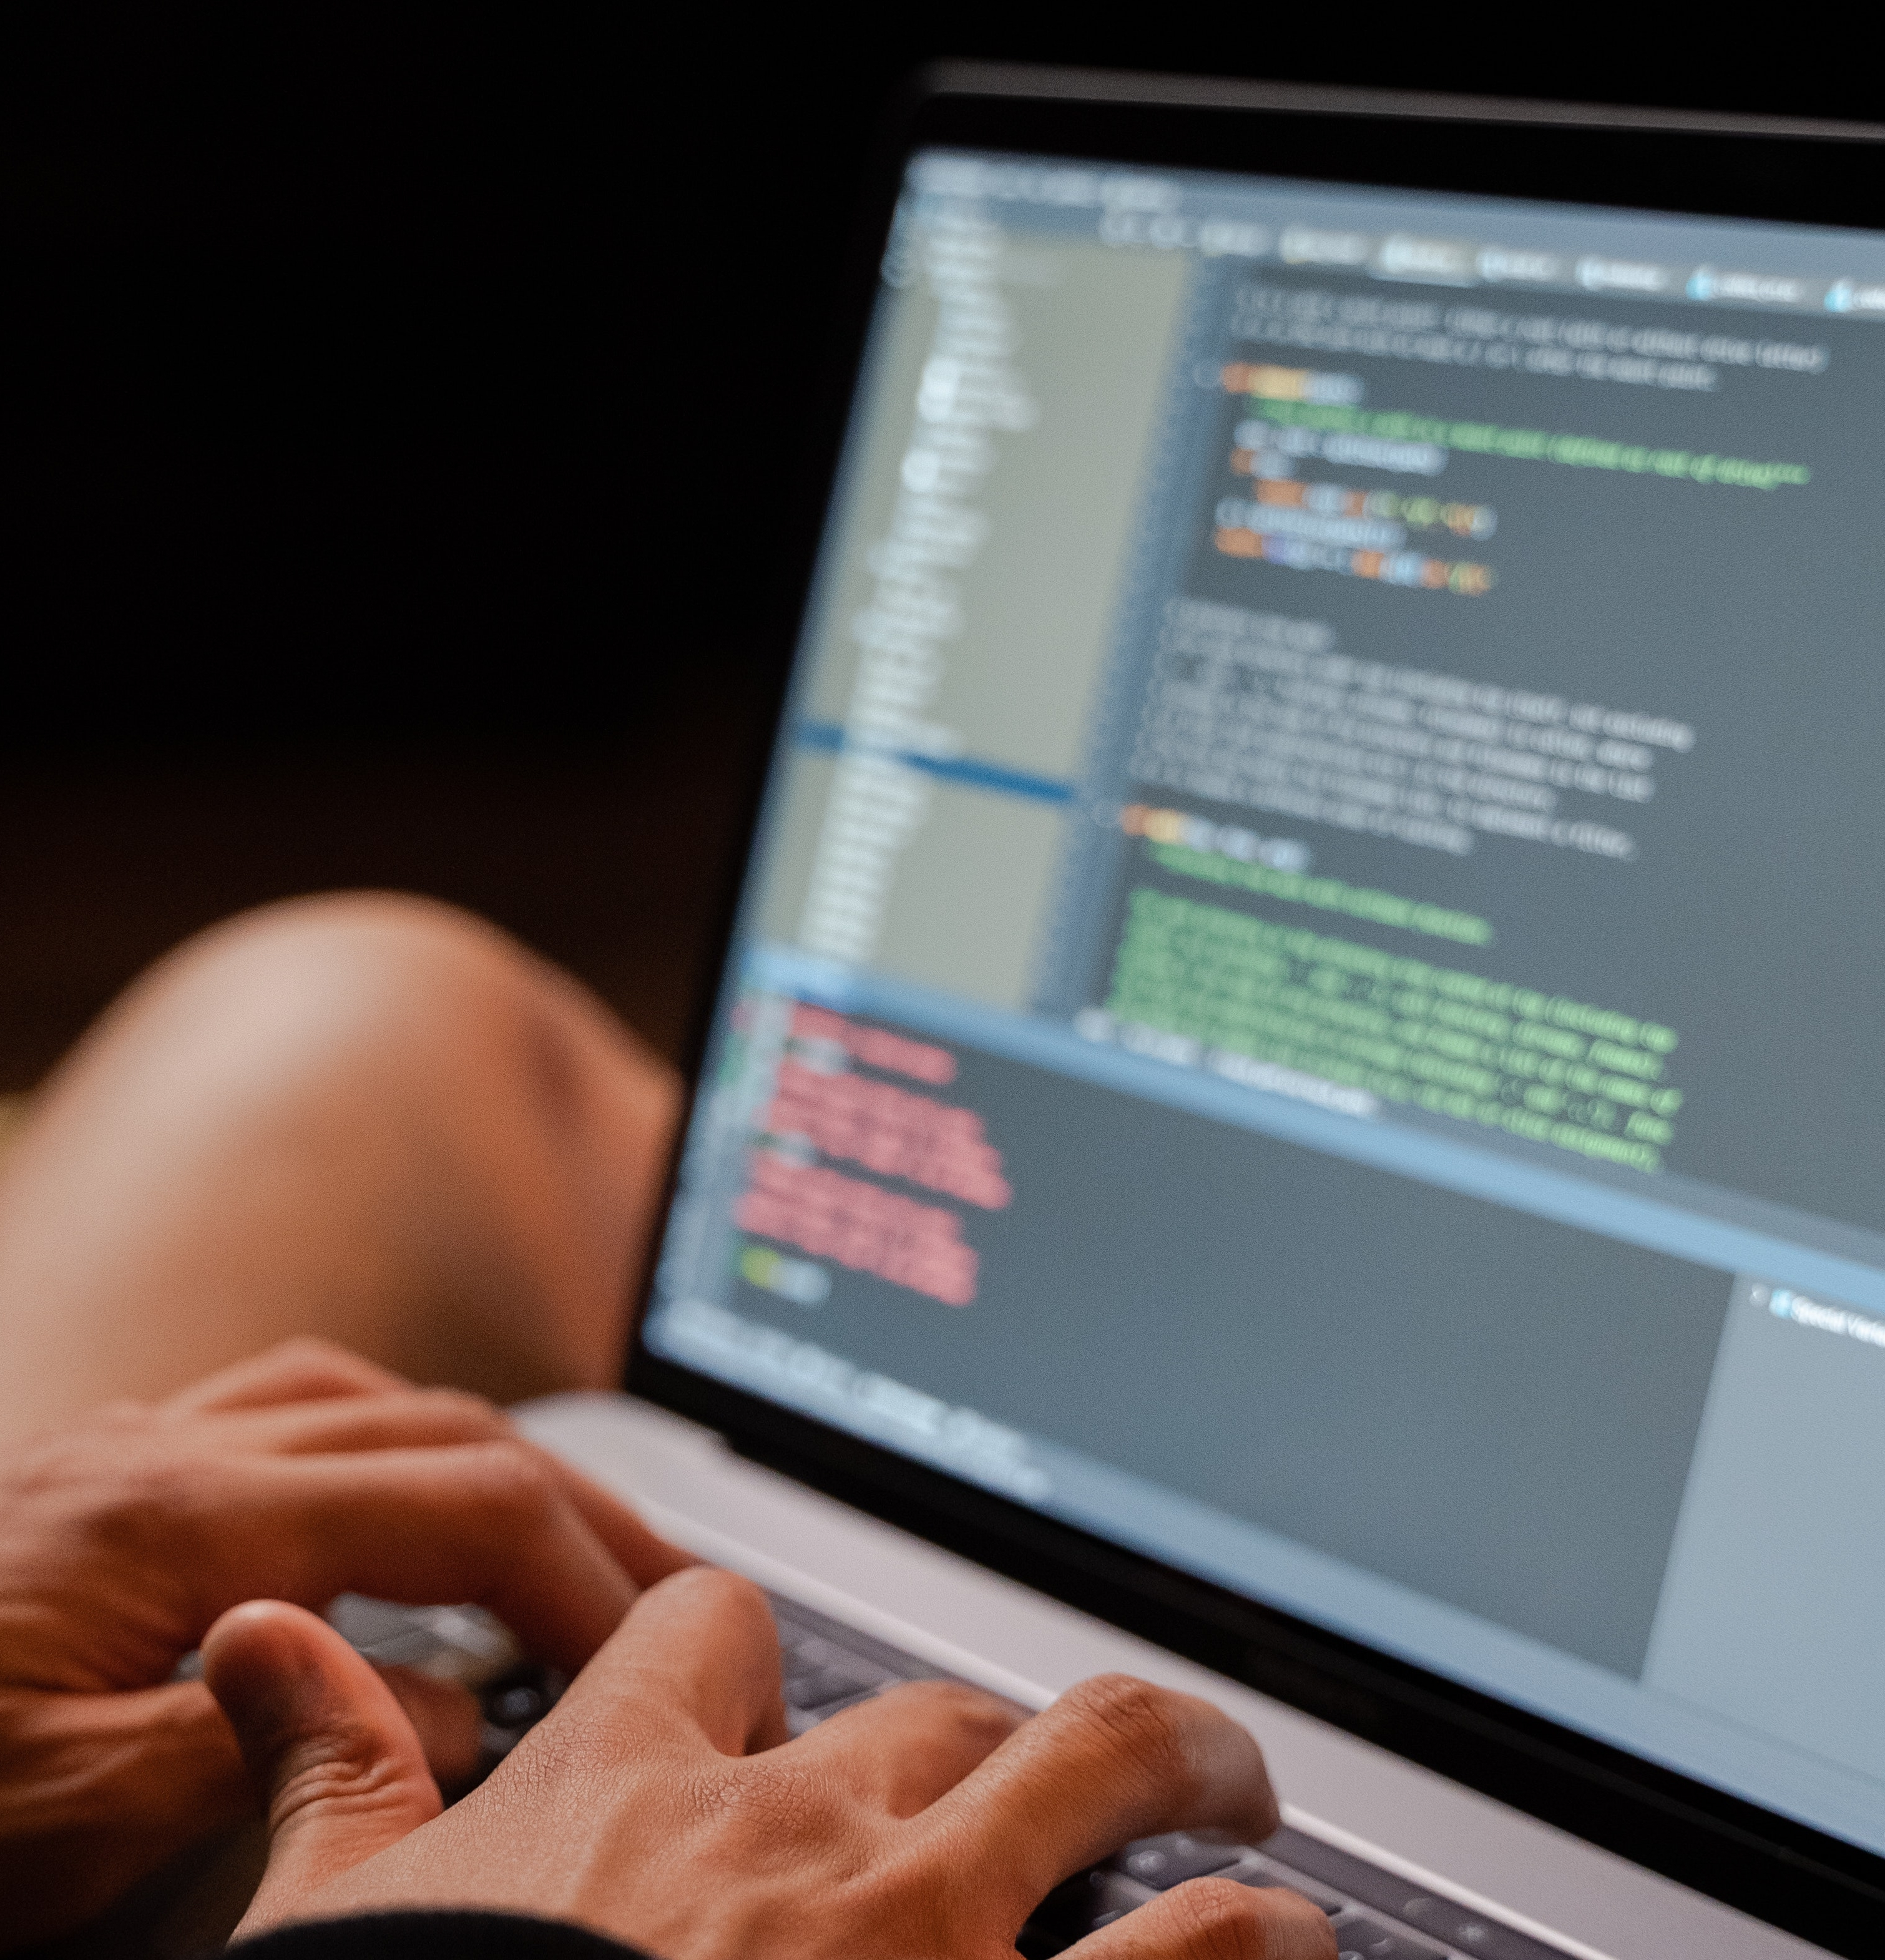
\includegraphics[width=0.6\linewidth]{./img/pc} 

}

\caption{Extraído de \href{https://images.pexels.com/photos/5496463/pexels-photo-5496463.jpeg?auto=compress&cs=tinysrgb&w=1260&h=750&dpr=1}{pixabay.com.}}\label{fig:unnamed-chunk-12}
\end{figure}

\endColumns
\end{frame}

\begin{frame}{Considerações}
\phantomsection\label{considerauxe7uxf5es}
\begin{itemize}
\item
  Onde há dados e incerteza, a Estatística pode ser usada.
\item
  A Estatística vai muito além do senso comum: tabelas e gráficos em
  revistas esportivas e jornais ou pesquisas de intenção de voto em
  épocas de eleição.
\item
  Existem diversas técnicas e possíveis áreas de aplicação.
\item
  A Estatística está por trás de boa parte do desenvolvimento científico
  moderno.
\end{itemize}
\end{frame}

\section{Algumas leituras
recomendadas}\label{algumas-leituras-recomendadas}

\begin{frame}{Livros técnicos}
\phantomsection\label{livros-tuxe9cnicos}
\beginAHalfColumn

\begin{figure}

{\centering \includegraphics[width=0.5\linewidth]{./img/noproest} 

}

\caption{Noções de Probabilidade e Estatística.}\label{fig:unnamed-chunk-13}
\end{figure}

\endColumns
\beginAHalfColumn

\begin{figure}

{\centering \includegraphics[width=0.5\linewidth]{./img/estbas} 

}

\caption{Estatística Básica.}\label{fig:unnamed-chunk-14}
\end{figure}

\endColumns
\end{frame}

\begin{frame}{Livros não técnicos}
\phantomsection\label{livros-nuxe3o-tuxe9cnicos}
\beginAHalfColumn

\begin{figure}

{\centering \includegraphics[width=0.5\linewidth]{./img/cha} 

}

\caption{Uma senhora toma chá.}\label{fig:unnamed-chunk-15}
\end{figure}

\endColumns
\beginAHalfColumn

\begin{figure}

{\centering \includegraphics[width=0.5\linewidth]{./img/bebado} 

}

\caption{O andar do bêbado.}\label{fig:unnamed-chunk-16}
\end{figure}

\endColumns
\end{frame}

\begin{frame}{Livros não técnicos}
\phantomsection\label{livros-nuxe3o-tuxe9cnicos-1}
\beginAHalfColumn

\begin{figure}

{\centering \includegraphics[width=0.5\linewidth]{./img/mentir} 

}

\caption{Como mentir com Estatística.}\label{fig:unnamed-chunk-17}
\end{figure}

\endColumns
\beginAHalfColumn

\begin{figure}

{\centering \includegraphics[width=0.5\linewidth]{./img/algoritmos} 

}

\caption{Algoritmos de destruição em massa.}\label{fig:unnamed-chunk-18}
\end{figure}

\endColumns
\end{frame}

\begin{frame}{Algumas frases para refletir}
\phantomsection\label{algumas-frases-para-refletir}
\beginTwoThirdsColumn

\emph{``Em Deus nós confiamos; todos os outros devem trazer dados.''}
William Edwards Deming

\vspace{1cm}

\emph{``O trabalho do estatístico é o de catalisar o processo de
construção do conhecimento científico.''} George E. P. Box

\vspace{1cm}

\emph{``A tentação de formular teorias prematuras sobre dados
insuficientes é a ruína da nossa profissão.''} Sherlock Holmes, de Sir
Arthur Conan Doyle

\endColumns\hfill
\beginAThirdColumn

\begin{center}\includegraphics[width=0.4\linewidth]{./img/deming} \end{center}

\begin{center}\includegraphics[width=0.4\linewidth]{./img/box} \end{center}

\begin{center}\includegraphics[width=0.4\linewidth]{./img/holmes} \end{center}

\endColumns
\end{frame}

\section{Dados}\label{dados}

\begin{frame}{O que são dados?}
\phantomsection\label{o-que-suxe3o-dados}
\beginAHalfColumn

\begin{itemize}
\tightlist
\item
  Dados são \textbf{conjuntos de valores}.
\end{itemize}

\vspace{0.3cm}

\begin{itemize}
\tightlist
\item
  Podem ser de diferentes fontes, tais como \textbf{estudos} e
  \textbf{experimentos}.
\end{itemize}

\vspace{0.3cm}

\begin{itemize}
\tightlist
\item
  Podem conter \textbf{variáveis} de diferentes tipos.
\end{itemize}

\vspace{0.3cm}

\begin{itemize}
\tightlist
\item
  Podem surgir em formatos \textbf{estruturados} e
  \textbf{não estruturados}.
\end{itemize}

\endColumns
\beginAHalfColumn

\begin{figure}

{\centering \includegraphics[width=0.9\linewidth]{./img/dados} 

}

\caption{Extraído de \href{https://cdn.pixabay.com/photo/2018/01/26/18/21/matrix-3109378_1280.jpg}{pixabay.com.}}\label{fig:unnamed-chunk-22}
\end{figure}

\endColumns
\end{frame}

\begin{frame}{Conjunto de dados}
\phantomsection\label{conjunto-de-dados}
\begin{itemize}
\item
  Em Estatística, em geral, lidamos com
  \textbf{dados estruturados em um formato tabular}.
\item
  Os dados nem sempre começam nessa forma. Muitas vezes a informação
  deve ser processada e tratada de modo a chegar nesta estrutura.
\item
  O conjunto de dados completo e sem tratamentos é denominado conjunto
  de \textbf{dados brutos}.
\end{itemize}

\vspace{0.3cm}

\begin{itemize}
\tightlist
\item
  Um conjunto de dados considerado \textbf{arrumado} é aquele em que:

  \begin{itemize}
  \tightlist
  \item
    Cada \textbf{coluna} representa uma \textbf{variável}.
  \item
    Cada \textbf{linha} representa uma \textbf{observação}.
  \item
    Cada \textbf{célula} representa o \textbf{valor} observado.
  \end{itemize}
\end{itemize}
\end{frame}

\begin{frame}{Conjunto de dados}
\phantomsection\label{conjunto-de-dados-1}
\begin{figure}

{\centering \includegraphics[width=0.9\linewidth]{./img/tidy-data} 

}

\caption{Adaptado de \href{https://r4ds.had.co.nz/tidy-data.html}{https://r4ds.had.co.nz}.}\label{fig:unnamed-chunk-23}
\end{figure}
\end{frame}

\begin{frame}{Conjunto de dados}
\phantomsection\label{conjunto-de-dados-2}
\begin{longtable}[]{@{}rllrrr@{}}
\caption{Exemplo de conjunto de dados}\tabularnewline
\toprule\noalign{}
ID & Sexo & Escolaridade & Altura & Peso & Irmãos \\
\midrule\noalign{}
\endfirsthead
\toprule\noalign{}
ID & Sexo & Escolaridade & Altura & Peso & Irmãos \\
\midrule\noalign{}
\endhead
1 & Masculino & Ensino superior & 182 & 80 & 0 \\
2 & Feminino & Ensino médio & 160 & 46 & 1 \\
3 & Feminino & Ensino superior & 160 & 55 & 4 \\
4 & Feminino & Mestrado & 165 & 58 & 3 \\
5 & Masculino & Ensino médio & 183 & 55 & 1 \\
\bottomrule\noalign{}
\end{longtable}
\end{frame}

\section{Fontes de dados}\label{fontes-de-dados}

\begin{frame}{De onde vêm os dados?}
\phantomsection\label{de-onde-vuxeam-os-dados}
\beginAHalfColumn

\textbf{Alguns exemplos}:

\begin{itemize}
\tightlist
\item
  Estudos de caso.
\item
  Experimentos.
\item
  Pesquisas.
\item
  Registros administrativos.
\item
  Dados em repositórios online.
\item
  Bancos de dados corporativos.
\item
  Sensores.
\item
  Textos, imagens e vídeos.
\end{itemize}

\endColumns
\beginAHalfColumn

\begin{figure}

{\centering \includegraphics[width=0.9\linewidth]{./img/fontes-dados} 

}

\caption{Extraído de \href{https://cdn.pixabay.com/photo/2022/03/02/09/37/data-7042739_1280.png}{pixabay.com.}}\label{fig:unnamed-chunk-25}
\end{figure}

\endColumns
\end{frame}

\begin{frame}{Dados observacionais x dados experimentais}
\phantomsection\label{dados-observacionais-x-dados-experimentais}
\beginAHalfColumn

\textbf{Dados observacionais}

\begin{itemize}
\tightlist
\item
  \textbf{Observação passiva} da realidade.
\item
  Sem modificação das condições.
\end{itemize}

\vspace{0.3cm}

\textbf{Dados experimentais}

\begin{itemize}
\tightlist
\item
  \textbf{Intervenção} na realidade.
\item
  Condições controladas.
\item
  Observação dos efeitos das intervenções.
\end{itemize}

\endColumns
\beginAHalfColumn

\begin{figure}

{\centering \includegraphics[width=0.9\linewidth]{./img/observar} 

}

\caption{Extraído de \href{https://cdn.pixabay.com/photo/2013/07/12/15/08/earth-149499_1280.png}{pixabay.com.}}\label{fig:unnamed-chunk-26}
\end{figure}

\endColumns
\end{frame}

\begin{frame}{Dados observacionais x dados experimentais}
\phantomsection\label{dados-observacionais-x-dados-experimentais-1}
\begin{itemize}
\item
  Cada tipo de estudo induz \textbf{relações} diferentes entre as
  observações e \textbf{modelos estatísticos} diferentes para modelar a
  incerteza destas relações.
\item
  Um \textbf{conjunto de dados} é um dos subprodutos de um estudo. Ele
  contém as características principais (variáveis) que se tem interesse
  em estudar em uma população ou amostra.
\item
  Estas características podem ser \textbf{qualitativas} ou
  \textbf{quantitativas} e a partir do conjunto de dados as análises
  inferenciais são feitas.
\item
  As variáveis são assim chamadas porque seus valores não são constantes
  e variam segundo regras ou leis naturais que podem ser conhecidas ou
  desconhecidas.
\end{itemize}
\end{frame}

\section{Tipos de variáveis}\label{tipos-de-variuxe1veis}

\begin{frame}{Tipos de variáveis}
\phantomsection\label{tipos-de-variuxe1veis-1}
\vspace{0.3cm}

\begin{itemize}
\item
  Na prática, podemos coletar variáveis de diferentes tipos e naturezas.
\item
  Antes de de qualquer análise precisamos ser capazes de compreender os
  tipos de variáveis pois estes tipos conduzirão às análises e métodos
  estatísticos que poderão ser aplicados.
\end{itemize}

\vspace{0.3cm}

\begin{itemize}
\tightlist
\item
  Existem dois tipos (básicos) de variáveis:

  \begin{itemize}
  \tightlist
  \item
    Numéricas (\textbf{quantitativas}).
  \item
    Não numéricas (\textbf{qualitativas}).
  \end{itemize}
\end{itemize}

\vspace{0.3cm}

\begin{figure}

{\centering \includegraphics[width=0.9\linewidth]{./img/tipos-variaveis2} 

}

\caption{Tipos básicos de variáveis.}\label{fig:unnamed-chunk-27}
\end{figure}
\end{frame}

\begin{frame}{Variáveis quantitativas}
\phantomsection\label{variuxe1veis-quantitativas}
\beginAHalfColumn

\begin{itemize}
\tightlist
\item
  \textbf{Variáveis Quantitativas}: assumem valores numéricos.

  \begin{itemize}
  \tightlist
  \item
    \textbf{Discretas}: características mensuráveis que podem assumir
    apenas um número finito ou infinito \textbf{contável} de valores.
  \item
    \textbf{Contínuas}: características mensuráveis que assumem valores
    em uma \textbf{escala contínua}, isto é, na reta real.
  \end{itemize}
\end{itemize}

\endColumns
\beginAHalfColumn

\textbf{Exemplos}

\begin{itemize}
\tightlist
\item
  Altura.
\item
  Peso.
\item
  Idade.
\item
  Percentual de gordura corporal.
\item
  Número de filhos.
\item
  Número de fraturas.
\item
  Número de faltas.
\item
  Número de peças defeituosas em um lote.
\end{itemize}

\endColumns
\end{frame}

\begin{frame}{Variáveis qualitativas}
\phantomsection\label{variuxe1veis-qualitativas}
\beginAHalfColumn

\begin{itemize}
\tightlist
\item
  \textbf{Variáveis Qualitativas}: são as características definidas por
  categorias, ou seja, representam uma classificação dos indivíduos e
  não uma característica numérica.

  \begin{itemize}
  \tightlist
  \item
    \textbf{Nominais}: não existe ordenação nem peso entre as
    categorias.
  \item
    \textbf{Ordinais}: existe uma ordenação entre as categorias.
  \end{itemize}
\end{itemize}

\endColumns
\beginAHalfColumn

\textbf{Exemplos}

\begin{itemize}
\tightlist
\item
  Estado civil.
\item
  Orientação sexual.
\item
  Turma.
\item
  Posição em que joga em um time.
\item
  Severidade de uma lesão.
\item
  Escolaridade.
\item
  Grau de proficiência em língua inglesa.
\item
  Risco de infarto.
\end{itemize}

\endColumns
\end{frame}

\begin{frame}{Cuidados com variáveis}
\phantomsection\label{cuidados-com-variuxe1veis}
\begin{itemize}
\tightlist
\item
  Existem particularidades na classificação de variáveis devido a
  situações como:

  \begin{itemize}
  \tightlist
  \item
    Discretização de variáveis contínuas.
  \item
    Limitações em instrumentos de mensuração.
  \item
    Utilização de quantidades numéricas para representação de variáveis
    categóricas.
  \item
    Dentre outras.
  \end{itemize}
\end{itemize}

\vspace{0.3cm}

\begin{itemize}
\item
  Deve-se sempre estar atento a este tipo de situação pois podem levar a
  implicações nas análises e consequentemente nos resultados.
\item
  Existem outros tipos de variáveis que ocorrem em situações
  particulares que requerem técnicas específicas de análise.
\end{itemize}
\end{frame}

\section{Análise de dados}\label{anuxe1lise-de-dados}

\begin{frame}{No que devemos pensar antes de analisar nossos dados?}
\phantomsection\label{no-que-devemos-pensar-antes-de-analisar-nossos-dados}
\begin{itemize}
\tightlist
\item
  O que estamos interessados em avaliar?
\item
  Quais são as variáveis de interesse?
\item
  Quais são as variáveis que queremos avaliar se influenciam a variável
  de interesse?
\item
  Quais são os métodos disponíveis para análise de variáveis deste tipo?
\item
  Quais os métodos disponíveis que permitem responder nossa pergunta de
  pesquisa?
\item
  Como coletar os dados?
\item
  Os dados são válidos?
\end{itemize}
\end{frame}

\section{Métodos de amostragem}\label{muxe9todos-de-amostragem}

\begin{frame}{Amostras}
\phantomsection\label{amostras}
\beginAHalfColumn

\begin{itemize}
\tightlist
\item
  Uma amostra é um \textbf{subconjunto da população}.
\end{itemize}

\vspace{0.3cm}

\begin{itemize}
\tightlist
\item
  Na prática costuma ser inviável trabalhar com a população toda.
\end{itemize}

\vspace{0.3cm}

\begin{itemize}
\tightlist
\item
  A alternativa então é trabalhar com uma \textbf{amostra} e
  \textbf{inferir} os resultados para a população.
\end{itemize}

\vspace{0.3cm}

\begin{itemize}
\tightlist
\item
  A seleção da amostra pode ser feita de diversas maneiras.
\end{itemize}

\endColumns
\beginAHalfColumn

\begin{figure}

{\centering \includegraphics[width=1\linewidth]{./img/populacao-amostra3} 

}

\caption{Extraído de \href{https://cdn.pixabay.com/photo/2017/10/25/18/18/rare-disease-2888820_1280.png}{pixabay.com.}}\label{fig:unnamed-chunk-28}
\end{figure}

\endColumns
\end{frame}

\begin{frame}{Amostras}
\phantomsection\label{amostras-1}
\beginAHalfColumn

\begin{itemize}
\tightlist
\item
  Os métodos de amostragem servem para selecionar subconjuntos da
  população de forma mais \textbf{representativa} possível.
\end{itemize}

\vspace{0.3cm}

\begin{itemize}
\tightlist
\item
  A forma adequada de amostragem conduz a um
  \textbf{menor tamanho amostral} para obtenção de uma
  \textbf{precisão satisfatória}.
\end{itemize}

\endColumns
\beginAHalfColumn

\begin{itemize}
\tightlist
\item
  São características desejáveis de uma amostra:

  \begin{itemize}
  \tightlist
  \item
    Capacidade de generalização.
  \item
    Imparcialidade e representatividade.
  \item
    Capacidade de medir a precisão das estimativas.
  \end{itemize}
\item
  Podemos dividir os métodos em:

  \begin{itemize}
  \tightlist
  \item
    Amostragem probabilística.
  \item
    Amostragem não probabilística.
  \end{itemize}
\end{itemize}

\endColumns
\end{frame}

\begin{frame}{Um caso clássico: a história do Literary Digest}
\phantomsection\label{um-caso-cluxe1ssico-a-histuxf3ria-do-literary-digest}
\begin{itemize}
\item
  O \textbf{Literary Digest} era uma revista americana de publicação
  semanal fundada em 1890.
\item
  Em 1936 ocorreu a 38ª \textbf{eleição presidencial} dos Estados
  Unidos.
\item
  Como candidatos haviam nomes como: Franklin Roosevelt, Alf Landon,
  William Lemke, Norman Thomas, dentre outros.
\item
  \textbf{Roosevelt} e \textbf{Landon} eram vistos como os favoritos.
\end{itemize}

\begin{figure}

{\centering \includegraphics[width=1\linewidth]{./img/1936} 

}

\caption{Franklin Roosevelt, Alf Landon, William Lemke e Norman Thomas.}\label{fig:unnamed-chunk-29}
\end{figure}
\end{frame}

\begin{frame}{Um caso clássico: a história do Literary Digest}
\phantomsection\label{um-caso-cluxe1ssico-a-histuxf3ria-do-literary-digest-1}
\begin{itemize}
\item
  No ano da eleição, o Literary Digest conduziu uma pesquisa de intenção
  de votos com \textbf{mais de 10 milhões de respondentes} com base em
  sua base de assinantes e outras listas de indivíduos.
\item
  Enquanto isso, George Gallup, fundador da Gallup Poll, conduziu
  pesquisas quinzenais com apenas \textbf{2 mil indivíduos}.
\item
  O Literary Digest previu a vitória de Landon, Gallup previu a vitória
  de Roosevelt. Qual dos dois acertou?
\end{itemize}
\end{frame}

\begin{frame}{Um caso clássico: a história do Literary Digest}
\phantomsection\label{um-caso-cluxe1ssico-a-histuxf3ria-do-literary-digest-2}
O resultado da eleição foi:

\begin{enumerate}
\tightlist
\item
  \textbf{Franklin D. Roosevelt, 27.752.648 de votos.}
\item
  Alf Landon, 16.681.862 de votos.
\item
  William Lemke, 892.378 votos.
\item
  Norman Thomas, 187.910 votos.
\item
  Outros, 132.901 votos.
\end{enumerate}

\vspace{0.5cm}

\begin{itemize}
\item
  Gallup acertou, Literary Digest errou.
\item
  O que deu errado na pesquisa do Literary Digest?

  \begin{itemize}
  \tightlist
  \item
    A resposta é: a \textbf{composição da amostra}.
  \end{itemize}
\end{itemize}
\end{frame}

\begin{frame}{Um caso clássico: a história do Literary Digest}
\phantomsection\label{um-caso-cluxe1ssico-a-histuxf3ria-do-literary-digest-3}
\begin{itemize}
\item
  O Literary Digest optou por \textbf{quantidade}, prestando pouca
  atenção ao método de seleção.
\item
  A amostra foi de \textbf{conveniência} e representava apenas o grupo
  da população com nível socioeconomico relativamente alto: seus
  próprios assinantes e pessoas que possuiam luxos da época como
  telefones.
\item
  Isso gerou um \textbf{viés de amostragem}, ou seja, a amostra era
  diferente, de modos importantes e não aleatórios, da população que
  deveria representar. Ou simplesmente:
  \textbf{a amostra não era representativa}.
\item
  Por outro lado, a amostra de Gallup era bem mais modesta, contudo o
  método de seleção gerou uma
  \textbf{amostra representativa da população} em que todas as camadas
  de votantes estavam presentes.
\end{itemize}
\end{frame}

\begin{frame}{Amostragem probabilística}
\phantomsection\label{amostragem-probabiluxedstica}
\beginAHalfColumn

\begin{itemize}
\tightlist
\item
  Amostragem probabilística deve ser usada \textbf{sempre que possível}.
\end{itemize}

\vspace{0.3cm}

\begin{itemize}
\tightlist
\item
  O objetivo é dimensionar amostras que sejam capazes de
  \textbf{estimar} as quantidades de interesse com uma certa
  \textbf{precisão} desejada.
\end{itemize}

\vspace{0.3cm}

\begin{itemize}
\tightlist
\item
  Existem diversos métodos disponíveis.
\end{itemize}

\endColumns
\beginAHalfColumn

\textbf{Alguns métodos são:}

\begin{itemize}
\tightlist
\item
  Amostragem aleatória simples (com ou sem reposição).
\item
  Amostragem sistemática.
\item
  Amostragem estratificada.
\item
  Amostragem por conglomerados.
\end{itemize}

\endColumns
\end{frame}

\begin{frame}{Amostragem não probabilística}
\phantomsection\label{amostragem-nuxe3o-probabiluxedstica}
\begin{itemize}
\item
  Em muitos casos não é possível fazer uso de métodos de amostragem
  probabilística.
\item
  Surgem então os métodos de amostragem não probabilística, como
  amostragem por conveniência, intencional/julgamento, bola de neve.
\item
  Uma avaliação da ``representatividade'' dos métodos de amostragem não
  probabilística não pode ser feita.
\item
  Devemos tomar muito cuidado ao interpretar resultados baseados em
  métodos de amostragem não probabilísticos.
\item
  Em geral, estas amostras carregam um alto risco de não serem
  representativas.
\item
  Não há métodos para análise probabilística ou inferencial dos
  resultados.
\end{itemize}
\end{frame}

\section{Análise exploratória}\label{anuxe1lise-exploratuxf3ria}

\begin{frame}{Análise exploratória}
\phantomsection\label{anuxe1lise-exploratuxf3ria-1}
\begin{itemize}
\item
  Parte primordial de qualquer análise estatística é chamada
  \textbf{análise descritiva} ou \textbf{exploratória}.
\item
  Consiste basicamente de \textbf{tabelas}, \textbf{resumos numéricos} e
  \textbf{análises gráficas} das variáveis disponíveis em um conjunto de
  dados.
\item
  Trata-se de uma etapa de extrema importância e deve preceder qualquer
  análise mais sofisticada.
\item
  As técnicas de análise exploratória visam \textbf{resumir} e
  \textbf{apresentar} as informações de um conjunto de dados brutos.
\end{itemize}
\end{frame}

\begin{frame}{Análise exploratória}
\phantomsection\label{anuxe1lise-exploratuxf3ria-2}
\beginAHalfColumn

\begin{itemize}
\tightlist
\item
  A análise exploratória de dados é uma área relativamente nova.
\end{itemize}

\vspace{0.3cm}

\begin{itemize}
\tightlist
\item
  Nasceu do clássico livro \textbf{Exploratory Data Analysis} de
  \textbf{John Tukey} em 1977.
\end{itemize}

\vspace{0.3cm}

\begin{itemize}
\tightlist
\item
  Algo curioso é que Tukey tinha uma relação próxima com a Ciência da
  Computação e definiu os termos \textbf{bit} e \textbf{software}.
\end{itemize}

\endColumns
\beginAHalfColumn

\begin{figure}

{\centering \includegraphics[width=0.62\linewidth]{./img/eda-tukey} 

}

\caption{Capa do livro Exploratory Data Analysis de John Tukey.}\label{fig:unnamed-chunk-30}
\end{figure}

\endColumns
\end{frame}

\begin{frame}{Análise exploratória}
\phantomsection\label{anuxe1lise-exploratuxf3ria-3}
\begin{itemize}
\item
  Como quase tudo em análise de dados, o \textbf{avanço computacional}
  permitiu com que a análise exploratória evoluísse substancialmente.
\item
  Por exemplo: historicamente o processo de criação de um gráfico era
  reservado a pessoas qualificadas pois a produção de uma visualização
  era difícil.
\item
  Hoje qualquer pessoa pode inserir dados em um aplicativo e gerar um
  gráfico.
\item
  Este tipo de facilidade é importante para disseminação e
  democratização dos métodos, porém abre margem para certas práticas
  inadequadas.
\end{itemize}
\end{frame}

\begin{frame}{Análise exploratória}
\phantomsection\label{anuxe1lise-exploratuxf3ria-4}
\beginAHalfColumn

\begin{itemize}
\tightlist
\item
  Tentar compreender um conjunto de dados sem algum método que permita
  resumir as informações é inviável.
\end{itemize}

\vspace{0.3cm}

\begin{itemize}
\tightlist
\item
  A análise exploratória é a primeira forma de tentarmos entender o que
  acontece nos nossos dados.
\end{itemize}

\vspace{0.3cm}

\begin{itemize}
\tightlist
\item
  Uma das tarefas é a etapa de consistência dos dados, isto é, verificar
  se os dados coletados são condizentes com a realidade.
\end{itemize}

\endColumns
\beginAHalfColumn

\begin{figure}

{\centering \includegraphics[width=0.9\linewidth]{./img/dados} 

}

\caption{Extraído de \href{https://cdn.pixabay.com/photo/2018/01/26/18/21/matrix-3109378_1280.jpg}{pixabay.com.}}\label{fig:unnamed-chunk-31}
\end{figure}

\endColumns
\end{frame}

\begin{frame}{Análise exploratória}
\phantomsection\label{anuxe1lise-exploratuxf3ria-5}
\beginAHalfColumn

\begin{itemize}
\tightlist
\item
  O conjunto de técnicas aplicáveis está diretamente associado ao
  \textbf{tipo das variáveis de interesse} (quantitativas x
  qualitativas) e suas ramificações.
\end{itemize}

\vspace{0.3cm}

\begin{itemize}
\tightlist
\item
  Podemos conduzir análises focadas nas variáveis uma a uma
  (\textbf{análises univariadas}).
\end{itemize}

\vspace{0.3cm}

\begin{itemize}
\tightlist
\item
  Também podemos conduzir análises focadas em avaliar a relação entre as
  variáveis (\textbf{análises multivariadas}).
\end{itemize}

\endColumns
\beginAHalfColumn

\begin{figure}

{\centering \includegraphics[width=0.8\linewidth]{./img/exploratoria} 

}

\caption{Extraído de \href{https://cdn.pixabay.com/photo/2020/08/03/10/00/graph-5459708_1280.png}{pixabay.com.}}\label{fig:unnamed-chunk-32}
\end{figure}

\endColumns
\end{frame}

\begin{frame}{Análise exploratória}
\phantomsection\label{anuxe1lise-exploratuxf3ria-6}
Podemos fazer uso diversas técnicas, tais como

\beginAHalfColumn

\begin{itemize}
\tightlist
\item
  Tabelas de frequência absolutas.
\item
  Tabelas de frequência relativas.
\item
  Tabelas de frequência acumuladas.
\item
  Tabelas para múltiplas variáveis.
\item
  Gráficos.
\end{itemize}

\endColumns
\beginAHalfColumn

\begin{itemize}
\tightlist
\item
  Medidas de posição central.
\item
  Medidas de posição relativa.
\item
  Medidas de forma.
\item
  Medidas de dispersão.
\item
  Medidas de associação.
\end{itemize}

\endColumns
\end{frame}

\begin{frame}{Análise exploratória}
\phantomsection\label{anuxe1lise-exploratuxf3ria-7}
\beginAHalfColumn

\begin{itemize}
\tightlist
\item
  Para ilustrar as técnicas de análise exploratória de dados, usaremos o
  conjunto de dados ``milsa''.
\end{itemize}

\vspace{0.3cm}

\begin{itemize}
\tightlist
\item
  Este conjunto de dados aparece no livro ``Estatística Básica'' de W.
  O. Bussab e P. A. Morettin.
\end{itemize}

\vspace{0.3cm}

\begin{itemize}
\tightlist
\item
  Conjunto de dados hipotético de atributos de 36 funcionários da
  companhia ``Milsa''.
\end{itemize}

\endColumns
\beginAHalfColumn

O conjunto possui as seguintes variáveis:

\begin{itemize}
\tightlist
\item
  \textbf{Funcionário}: identificadora de funcionário.
\item
  \textbf{Estado civil}: casado ou solteiro.
\item
  \textbf{Instrução}: 1º grau, 2º grau, superior.
\item
  \textbf{Filhos}: número de filhos.
\item
  \textbf{Salário}: salário do funcionário.
\item
  \textbf{Anos}: idade em anos completos.
\item
  \textbf{Meses}: meses além dos anos completos.
\item
  \textbf{Região}: capital, interior, outro.
\end{itemize}

\endColumns
\end{frame}

\begin{frame}{Análise exploratória}
\phantomsection\label{anuxe1lise-exploratuxf3ria-8}
\begin{longtable}[]{@{}
  >{\centering\arraybackslash}p{(\columnwidth - 14\tabcolsep) * \real{0.1667}}
  >{\centering\arraybackslash}p{(\columnwidth - 14\tabcolsep) * \real{0.1795}}
  >{\centering\arraybackslash}p{(\columnwidth - 14\tabcolsep) * \real{0.1410}}
  >{\centering\arraybackslash}p{(\columnwidth - 14\tabcolsep) * \real{0.1026}}
  >{\centering\arraybackslash}p{(\columnwidth - 14\tabcolsep) * \real{0.1154}}
  >{\centering\arraybackslash}p{(\columnwidth - 14\tabcolsep) * \real{0.0769}}
  >{\centering\arraybackslash}p{(\columnwidth - 14\tabcolsep) * \real{0.0897}}
  >{\centering\arraybackslash}p{(\columnwidth - 14\tabcolsep) * \real{0.1282}}@{}}
\caption{Primeiras linhas do conjunto de dados Milsa.}\tabularnewline
\toprule\noalign{}
\begin{minipage}[b]{\linewidth}\centering
Funcionário
\end{minipage} & \begin{minipage}[b]{\linewidth}\centering
Estado civil
\end{minipage} & \begin{minipage}[b]{\linewidth}\centering
Instrução
\end{minipage} & \begin{minipage}[b]{\linewidth}\centering
Filhos
\end{minipage} & \begin{minipage}[b]{\linewidth}\centering
Salário
\end{minipage} & \begin{minipage}[b]{\linewidth}\centering
Anos
\end{minipage} & \begin{minipage}[b]{\linewidth}\centering
Meses
\end{minipage} & \begin{minipage}[b]{\linewidth}\centering
Região
\end{minipage} \\
\midrule\noalign{}
\endfirsthead
\toprule\noalign{}
\begin{minipage}[b]{\linewidth}\centering
Funcionário
\end{minipage} & \begin{minipage}[b]{\linewidth}\centering
Estado civil
\end{minipage} & \begin{minipage}[b]{\linewidth}\centering
Instrução
\end{minipage} & \begin{minipage}[b]{\linewidth}\centering
Filhos
\end{minipage} & \begin{minipage}[b]{\linewidth}\centering
Salário
\end{minipage} & \begin{minipage}[b]{\linewidth}\centering
Anos
\end{minipage} & \begin{minipage}[b]{\linewidth}\centering
Meses
\end{minipage} & \begin{minipage}[b]{\linewidth}\centering
Região
\end{minipage} \\
\midrule\noalign{}
\endhead
1 & solteiro & 1o Grau & NA & 4.00 & 26 & 3 & interior \\
2 & casado & 1o Grau & 1 & 4.56 & 32 & 10 & capital \\
3 & casado & 1o Grau & 2 & 5.25 & 36 & 5 & capital \\
4 & solteiro & 2o Grau & NA & 5.73 & 20 & 10 & outro \\
5 & solteiro & 1o Grau & NA & 6.26 & 40 & 7 & outro \\
6 & casado & 1o Grau & 0 & 6.66 & 28 & 0 & interior \\
7 & solteiro & 1o Grau & NA & 6.86 & 41 & 0 & interior \\
8 & solteiro & 1o Grau & NA & 7.39 & 43 & 4 & capital \\
9 & casado & 2o Grau & 1 & 7.59 & 34 & 10 & capital \\
10 & solteiro & 2o Grau & NA & 7.44 & 23 & 6 & outro \\
\bottomrule\noalign{}
\end{longtable}
\end{frame}

\section{Análise descritiva univariada para variáveis
qualitativas}\label{anuxe1lise-descritiva-univariada-para-variuxe1veis-qualitativas}

\begin{frame}{Análise descritiva univariada para variáveis qualitativas}
\phantomsection\label{anuxe1lise-descritiva-univariada-para-variuxe1veis-qualitativas-1}
\begin{itemize}
\item
  Uma variável qualitativa representa um atributo que pode ser expresso
  por meio de \textbf{rótulos} ou \textbf{categorias}.
\item
  Podem ser classificadas em \textbf{nominais} (sem ordenação natural
  entre as categorias) ou \textbf{ordinais} (com ordenação natural entre
  as categorias).
\item
  As categorias também são chamadas de \textbf{classes} ou
  \textbf{níveis}.
\item
  Na análise descritiva de uma variável qualitativa estamos interessados
  em avaliar as \textbf{frequências} das classes.
\end{itemize}
\end{frame}

\begin{frame}{Tipos de frequência}
\phantomsection\label{tipos-de-frequuxeancia}
\begin{itemize}
\item
  \textbf{Frequência absoluta} (\(f_a\)): número de observações no
  conjunto de dados que pertence a uma determinada classe.
\item
  \textbf{Frequência relativa} (\(f_r\)): frequência de classe dividida
  pelo número total de observações no conjunto de dados.

  \begin{itemize}
  \tightlist
  \item
    Pode ser apresentada em forma de percentual, quando multiplicada por
    100.
  \end{itemize}
\item
  \textbf{Frequência acumulada} (\(F_a\) ou \(F_r\)): frequência
  absoluta ou relativa acumulada conforme disposição das classes.

  \begin{itemize}
  \tightlist
  \item
    Não faz muito sentido para variáveis qualitativas nominais.
  \end{itemize}
\end{itemize}
\end{frame}

\begin{frame}{Tabelas de frequência para uma variável qualitativa}
\phantomsection\label{tabelas-de-frequuxeancia-para-uma-variuxe1vel-qualitativa}
\beginAHalfColumn

\begin{itemize}
\tightlist
\item
  Utlizando apenas os dados brutos é difícil responder questões de
  interesse.
\end{itemize}

\vspace{0.3cm}

\begin{itemize}
\tightlist
\item
  Para reduzir os dados originais de forma que fique mais claro o
  entendimento dos mesmos são utilizadas as
  \textbf{tabelas de frequência}.
\end{itemize}

\vspace{0.3cm}

\begin{itemize}
\tightlist
\item
  No caso de variáveis qualitativas consiste em listar os possíveis
  níveis da variável e fazer a contagem de quantas vezes cada nível
  aparece nos dados brutos.
\end{itemize}

\endColumns
\beginAHalfColumn

\begin{figure}

{\centering \includegraphics[width=0.4\linewidth]{./img/tabela} 

}

\caption{Extraído de \href{https://cdn.pixabay.com/photo/2016/12/11/01/28/spreadsheet-icon-1898557_1280.png}{pixabay.com.}}\label{fig:unnamed-chunk-34}
\end{figure}

\endColumns
\end{frame}

\begin{frame}{Tabelas de frequência para uma variável qualitativa}
\phantomsection\label{tabelas-de-frequuxeancia-para-uma-variuxe1vel-qualitativa-1}
\begin{itemize}
\item
  Cada \textbf{linha} da tabela diz respeito a um \textbf{nível} da
  variável.
\item
  As \textbf{colunas} podem apresentar diferentes tipos de
  \textbf{frequência} (absoluta, relativa).
\item
  Alguns cuidados para a apresentação dos resultados dizem respeito ao
  tipo de variável em questão: nominal ou ordinal.
\item
  Os níveis de variáveis
  \textbf{nominais não apresentam uma ordenação natural}, portanto, na
  apresentação dos resultados pode ser interessante \textbf{ordenar} os
  níveis \textbf{por frequência} ou \textbf{por ordem alfabética}.
\item
  Esta estratégia não é recomendada para variáveis \textbf{ordinais},
  pois estas \textbf{apresentam uma ordenação natural} e esta ordenação
  deve ser preferencialmente mantida na exposição dos resultados.
\end{itemize}
\end{frame}

\begin{frame}{Tabelas de frequência para uma variável qualitativa
nominal}
\phantomsection\label{tabelas-de-frequuxeancia-para-uma-variuxe1vel-qualitativa-nominal}
\begin{longtable}[]{@{}ccc@{}}
\caption{Tabela de frequências para a região.}\tabularnewline
\toprule\noalign{}
Região & Frequência & Freq. Relativa \\
\midrule\noalign{}
\endfirsthead
\toprule\noalign{}
Região & Frequência & Freq. Relativa \\
\midrule\noalign{}
\endhead
capital & 11 & 0.31 \\
interior & 12 & 0.33 \\
outro & 13 & 0.36 \\
Total & 36 & 1.00 \\
\bottomrule\noalign{}
\end{longtable}
\end{frame}

\begin{frame}{Tabelas de frequência para uma variável qualitativa
nominal}
\phantomsection\label{tabelas-de-frequuxeancia-para-uma-variuxe1vel-qualitativa-nominal-1}
\begin{longtable}[]{@{}ccc@{}}
\caption{Tabela de frequências para a região.}\tabularnewline
\toprule\noalign{}
Região & Frequência & Freq. Relativa \\
\midrule\noalign{}
\endfirsthead
\toprule\noalign{}
Região & Frequência & Freq. Relativa \\
\midrule\noalign{}
\endhead
outro & 13 & 0.36 \\
interior & 12 & 0.33 \\
capital & 11 & 0.31 \\
Total & 36 & 1.00 \\
\bottomrule\noalign{}
\end{longtable}
\end{frame}

\begin{frame}{Tabelas de frequência para uma variável qualitativa
nominal}
\phantomsection\label{tabelas-de-frequuxeancia-para-uma-variuxe1vel-qualitativa-nominal-2}
\begin{longtable}[]{@{}ccc@{}}
\caption{Tabela de frequências para a região.}\tabularnewline
\toprule\noalign{}
Região & Frequência & Percentual \\
\midrule\noalign{}
\endfirsthead
\toprule\noalign{}
Região & Frequência & Percentual \\
\midrule\noalign{}
\endhead
outro & 13 & 36 \% \\
interior & 12 & 33 \% \\
capital & 11 & 31 \% \\
Total & 36 & 100 \% \\
\bottomrule\noalign{}
\end{longtable}
\end{frame}

\begin{frame}{Tabelas de frequência para uma variável qualitativa
ordinal}
\phantomsection\label{tabelas-de-frequuxeancia-para-uma-variuxe1vel-qualitativa-ordinal}
\begin{longtable}[]{@{}
  >{\centering\arraybackslash}p{(\columnwidth - 8\tabcolsep) * \real{0.1410}}
  >{\centering\arraybackslash}p{(\columnwidth - 8\tabcolsep) * \real{0.1538}}
  >{\centering\arraybackslash}p{(\columnwidth - 8\tabcolsep) * \real{0.2051}}
  >{\centering\arraybackslash}p{(\columnwidth - 8\tabcolsep) * \real{0.2179}}
  >{\centering\arraybackslash}p{(\columnwidth - 8\tabcolsep) * \real{0.2821}}@{}}
\caption{Tabela de frequências para o grau de instrução.}\tabularnewline
\toprule\noalign{}
\begin{minipage}[b]{\linewidth}\centering
Instrução
\end{minipage} & \begin{minipage}[b]{\linewidth}\centering
Frequência
\end{minipage} & \begin{minipage}[b]{\linewidth}\centering
Freq. Relativa
\end{minipage} & \begin{minipage}[b]{\linewidth}\centering
Freq. Acumulada
\end{minipage} & \begin{minipage}[b]{\linewidth}\centering
Freq. Rel. Acumulada
\end{minipage} \\
\midrule\noalign{}
\endfirsthead
\toprule\noalign{}
\begin{minipage}[b]{\linewidth}\centering
Instrução
\end{minipage} & \begin{minipage}[b]{\linewidth}\centering
Frequência
\end{minipage} & \begin{minipage}[b]{\linewidth}\centering
Freq. Relativa
\end{minipage} & \begin{minipage}[b]{\linewidth}\centering
Freq. Acumulada
\end{minipage} & \begin{minipage}[b]{\linewidth}\centering
Freq. Rel. Acumulada
\end{minipage} \\
\midrule\noalign{}
\endhead
1o Grau & 12 & 0.33 & 12 & 0.33 \\
2o Grau & 18 & 0.50 & 30 & 0.83 \\
Superior & 6 & 0.17 & 36 & 1.00 \\
Total & 36 & 1.00 & 36 & 1.00 \\
\bottomrule\noalign{}
\end{longtable}
\end{frame}

\begin{frame}{Tabelas de frequência para uma variável qualitativa
ordinal}
\phantomsection\label{tabelas-de-frequuxeancia-para-uma-variuxe1vel-qualitativa-ordinal-1}
\begin{longtable}[]{@{}
  >{\centering\arraybackslash}p{(\columnwidth - 8\tabcolsep) * \real{0.1486}}
  >{\centering\arraybackslash}p{(\columnwidth - 8\tabcolsep) * \real{0.1622}}
  >{\centering\arraybackslash}p{(\columnwidth - 8\tabcolsep) * \real{0.1622}}
  >{\centering\arraybackslash}p{(\columnwidth - 8\tabcolsep) * \real{0.2297}}
  >{\centering\arraybackslash}p{(\columnwidth - 8\tabcolsep) * \real{0.2973}}@{}}
\caption{Tabela de frequências para o grau de instrução.}\tabularnewline
\toprule\noalign{}
\begin{minipage}[b]{\linewidth}\centering
Instrução
\end{minipage} & \begin{minipage}[b]{\linewidth}\centering
Frequência
\end{minipage} & \begin{minipage}[b]{\linewidth}\centering
Percentual
\end{minipage} & \begin{minipage}[b]{\linewidth}\centering
Freq. Acumulada
\end{minipage} & \begin{minipage}[b]{\linewidth}\centering
Percentual Acumulado
\end{minipage} \\
\midrule\noalign{}
\endfirsthead
\toprule\noalign{}
\begin{minipage}[b]{\linewidth}\centering
Instrução
\end{minipage} & \begin{minipage}[b]{\linewidth}\centering
Frequência
\end{minipage} & \begin{minipage}[b]{\linewidth}\centering
Percentual
\end{minipage} & \begin{minipage}[b]{\linewidth}\centering
Freq. Acumulada
\end{minipage} & \begin{minipage}[b]{\linewidth}\centering
Percentual Acumulado
\end{minipage} \\
\midrule\noalign{}
\endhead
1o Grau & 12 & 33 \% & 12 & 33 \% \\
2o Grau & 18 & 50 \% & 30 & 83 \% \\
Superior & 6 & 17 \% & 36 & 100 \% \\
Total & 36 & 100 \% & 36 & 100 \% \\
\bottomrule\noalign{}
\end{longtable}
\end{frame}

\begin{frame}{Gráficos para representação de frequências de uma variável
qualitativa}
\phantomsection\label{gruxe1ficos-para-representauxe7uxe3o-de-frequuxeancias-de-uma-variuxe1vel-qualitativa}
\beginAHalfColumn

\begin{itemize}
\tightlist
\item
  A representação por meio de tabelas é útil mas nem sempre eficiente.
\end{itemize}

\vspace{0.3cm}

\begin{itemize}
\tightlist
\item
  Em diversos casos pode ser mais conveniente utilizar um
  \textbf{gráfico}.
\end{itemize}

\vspace{0.3cm}

\begin{itemize}
\tightlist
\item
  ``Uma imagem vale mais que mil palavras''.
\end{itemize}

\vspace{0.3cm}

\begin{itemize}
\tightlist
\item
  Os cuidados com a ordenação dos níveis de acordo com o tipo da
  variável se mantém.
\end{itemize}

\endColumns
\beginAHalfColumn

Algumas possibilidades são:

\begin{itemize}
\tightlist
\item
  Gráfico de barras verticais.
\item
  Gráfico de barras horizontais.
\item
  Gráfico de barras empilhadas.
\item
  Gráfico de setores.
\end{itemize}

\endColumns
\end{frame}

\begin{frame}{Gráfico de barras}
\phantomsection\label{gruxe1fico-de-barras}
\textbf{Gráfico de barras verticais ou horizontais.}

\begin{itemize}
\tightlist
\item
  Utiliza os possíveis \textbf{níveis} das variáveis
  \textbf{em um eixo}.
\item
  As \textbf{frequências ou porcentagens} ficam \textbf{no outro eixo}.
\item
  O tamanho da barra corresponde à frequência ou percentual.
\end{itemize}

\vspace{0.5cm}

\textbf{Gráfico de barras empilhadas}.

\begin{itemize}
\tightlist
\item
  Usa-se \textbf{uma única barra}.
\item
  A barra é dividida de acordo com a \textbf{contribuição relativa} de
  cada nível da variável.
\item
  Representa-se a frequência relativa ou o percentual.
\end{itemize}
\end{frame}

\begin{frame}{Gráfico de barras verticais}
\phantomsection\label{gruxe1fico-de-barras-verticais}
\begin{figure}

{\centering \includegraphics[width=11cm]{encontro1_files/figure-beamer/unnamed-chunk-40-1} 

}

\caption{Gráfico de barras verticais para a região.}\label{fig:unnamed-chunk-40}
\end{figure}
\end{frame}

\begin{frame}{Gráfico de barras verticais}
\phantomsection\label{gruxe1fico-de-barras-verticais-1}
\begin{figure}

{\centering \includegraphics[width=11cm]{encontro1_files/figure-beamer/unnamed-chunk-41-1} 

}

\caption{Gráfico de barras verticais para a região.}\label{fig:unnamed-chunk-41}
\end{figure}
\end{frame}

\begin{frame}{Gráfico de barras horizontais}
\phantomsection\label{gruxe1fico-de-barras-horizontais}
\begin{figure}

{\centering \includegraphics[width=11cm]{encontro1_files/figure-beamer/unnamed-chunk-42-1} 

}

\caption{Gráfico de barras horizontais para a região.}\label{fig:unnamed-chunk-42}
\end{figure}
\end{frame}

\begin{frame}{Gráfico de barras empilhadas}
\phantomsection\label{gruxe1fico-de-barras-empilhadas}
\begin{figure}

{\centering \includegraphics[width=11cm]{encontro1_files/figure-beamer/unnamed-chunk-43-1} 

}

\caption{Gráfico de barras empilhadas para a região.}\label{fig:unnamed-chunk-43}
\end{figure}
\end{frame}

\begin{frame}{Gráfico de setores}
\phantomsection\label{gruxe1fico-de-setores}
\begin{itemize}
\tightlist
\item
  Consiste em \textbf{repartir um círculo} em setores de tamanhos
  proporcionais às \textbf{frequências relativas} ou às
  \textbf{porcentagens} de cada valor.
\item
  Pode ser usados para representar variáveis com \textbf{poucos níveis}.
\item
  Apesar de muito usado e preferido em diversas áreas,
  \textbf{deve ser evitado}.
\item
  O cérebro humano tem dificuldade em relacionar \textbf{frequências}
  com \textbf{áreas relativas}.
\item
  Para variáveis com muitos níveis, o gráfico tende a ficar
  \textbf{visualmente poluído} e \textbf{pouco informativo}.
\item
  Outro problema é que níveis com
  \textbf{frequências iguais a 0 deixam de aparecer no gráfico},
  diferente de um gráfico de barras.
\end{itemize}
\end{frame}

\begin{frame}{Gráfico de setores}
\phantomsection\label{gruxe1fico-de-setores-1}
\begin{figure}

{\centering \includegraphics[width=11cm]{encontro1_files/figure-beamer/unnamed-chunk-44-1} 

}

\caption{Gráfico de setores para a região}\label{fig:unnamed-chunk-44}
\end{figure}
\end{frame}

\section{Análise descritiva univariada para variáveis
quantitativas}\label{anuxe1lise-descritiva-univariada-para-variuxe1veis-quantitativas}

\begin{frame}{Análise descritiva univariada para variáveis
quantitativas}
\phantomsection\label{anuxe1lise-descritiva-univariada-para-variuxe1veis-quantitativas-1}
\begin{itemize}
\item
  Uma variável quantitativa é uma \textbf{característica} que pode ser
  \textbf{mensurada} e representada \textbf{numericamente}.
\item
  Podem ser classificadas em \textbf{discretas} (finitos valores em um
  dado intervalo) ou \textbf{contínuas} (infinitos valores em um dado
  intervalo).
\item
  Quando estamos lidando com
  \textbf{variáveis quantitativas discretas com poucos possíveis valores},
  as técnicas apresentadas para variáveis qualitativas se aplicam.
\end{itemize}
\end{frame}

\begin{frame}{Tabelas de frequência}
\phantomsection\label{tabelas-de-frequuxeancia}
\begin{longtable}[]{@{}
  >{\centering\arraybackslash}p{(\columnwidth - 8\tabcolsep) * \real{0.1127}}
  >{\centering\arraybackslash}p{(\columnwidth - 8\tabcolsep) * \real{0.1690}}
  >{\centering\arraybackslash}p{(\columnwidth - 8\tabcolsep) * \real{0.1690}}
  >{\centering\arraybackslash}p{(\columnwidth - 8\tabcolsep) * \real{0.2394}}
  >{\centering\arraybackslash}p{(\columnwidth - 8\tabcolsep) * \real{0.3099}}@{}}
\caption{Tabela de frequências para o número de filhos (desconsiderando
dados ausentes).}\tabularnewline
\toprule\noalign{}
\begin{minipage}[b]{\linewidth}\centering
Filhos
\end{minipage} & \begin{minipage}[b]{\linewidth}\centering
Frequência
\end{minipage} & \begin{minipage}[b]{\linewidth}\centering
Percentual
\end{minipage} & \begin{minipage}[b]{\linewidth}\centering
Freq. Acumulada
\end{minipage} & \begin{minipage}[b]{\linewidth}\centering
Percentual Acumulado
\end{minipage} \\
\midrule\noalign{}
\endfirsthead
\toprule\noalign{}
\begin{minipage}[b]{\linewidth}\centering
Filhos
\end{minipage} & \begin{minipage}[b]{\linewidth}\centering
Frequência
\end{minipage} & \begin{minipage}[b]{\linewidth}\centering
Percentual
\end{minipage} & \begin{minipage}[b]{\linewidth}\centering
Freq. Acumulada
\end{minipage} & \begin{minipage}[b]{\linewidth}\centering
Percentual Acumulado
\end{minipage} \\
\midrule\noalign{}
\endhead
0 & 4 & 20 \% & 4 & 20 \% \\
1 & 5 & 25 \% & 9 & 45 \% \\
2 & 7 & 35 \% & 16 & 80 \% \\
3 & 3 & 15 \% & 19 & 95 \% \\
4 & 0 & 0 \% & 19 & 95 \% \\
5 & 1 & 5 \% & 20 & 100 \% \\
Total & 20 & 100 \% & 20 & 100 \% \\
\bottomrule\noalign{}
\end{longtable}
\end{frame}

\begin{frame}{Gráfico de barras verticais}
\phantomsection\label{gruxe1fico-de-barras-verticais-2}
\begin{figure}

{\centering \includegraphics[width=11cm]{encontro1_files/figure-beamer/unnamed-chunk-46-1} 

}

\caption{Gráfico de barras verticais para o número de filhos.}\label{fig:unnamed-chunk-46}
\end{figure}
\end{frame}

\begin{frame}{Análise descritiva univariada para variáveis
quantitativas}
\phantomsection\label{anuxe1lise-descritiva-univariada-para-variuxe1veis-quantitativas-2}
\begin{itemize}
\item
  Para variáveis quantitativas \textbf{contínuas} ou
  \textbf{discretas com muitos possíveis valores}, precisamos de
  técnicas específicas.
\item
  Uma estratégia comum é o \textbf{agrupamento em faixas de valores}, e
  avaliação das frequências nestas faixas.
\item
  Podem ser usadas \textbf{tabelas de frequências} absolutas, relativas
  e acumuladas para as faixas de valores.
\item
  Utilizando a
  \textbf{razão entre frequência relativa e a amplitude das faixas} de
  valores, geramos a \textbf{densidade}.
\end{itemize}
\end{frame}

\begin{frame}{Análise descritiva univariada para variáveis
quantitativas}
\phantomsection\label{anuxe1lise-descritiva-univariada-para-variuxe1veis-quantitativas-3}
\textbf{Faixas de valores}

\beginAHalfColumn

\begin{itemize}
\tightlist
\item
  Cuidados devem ser tomados quanto às notações e tipos de faixas
  (aberto e fechado à esquerda ou direita).
\end{itemize}

\vspace{0.5cm}

\begin{itemize}
\tightlist
\item
  Diferentes pessoas e softwares podem usar intervalos distintos.
\end{itemize}

\vspace{0.5cm}

\begin{itemize}
\tightlist
\item
  Em geral usaremos intervalos \textbf{fechados à esquerda} e
  \textbf{abertos à direita}.
\end{itemize}

\vspace{0.5cm}

\begin{itemize}
\tightlist
\item
  Considerando dois valores \(a\) e \(b\), em que \(a < b\), os
  intervalos consideram que \(a\) \textbf{não} está incluído na faixa,
  \(b\) está.
\end{itemize}

\endColumns
\beginAHalfColumn

\begin{itemize}
\tightlist
\item
  Notações usuais:

  \begin{itemize}
  \tightlist
  \item
    \(a \leq y < b\).
  \item
    \(a \vdash b\).
  \item
    \([a,b)\).
  \item
    \([a,b[\).
  \end{itemize}
\item
  Exemplo:

  \begin{itemize}
  \tightlist
  \item
    \(5 \leq y < 10\).
  \item
    \(5 \vdash 10\).
  \item
    \([5,10)\).
  \item
    \([5,10[\).
  \item
    Valores maiores ou iguais a 5 até valores menores que 10 (10 não
    está no intervalo).
  \end{itemize}
\end{itemize}

\endColumns
\end{frame}

\begin{frame}{Análise descritiva univariada para variáveis
quantitativas}
\phantomsection\label{anuxe1lise-descritiva-univariada-para-variuxe1veis-quantitativas-4}
Perguntas que surgem são:

\begin{itemize}
\item
  Como agrupar em classes?
\item
  Qual o tamanho ideal das faixas de valores?
\end{itemize}

\vspace{0.5cm}

\begin{itemize}
\item
  Classes definidas com a \textbf{mesma amplitude} é o procedimento mais
  usual, apesar de ser possível definir classes com tamanhos diferentes.
\item
  Existem procedimentos que podem ser usados para obter a amplitude,
  como \textbf{Sturges}.
\item
  Em geral, \textbf{5} a \textbf{15} faixas são suficientes.
\end{itemize}
\end{frame}

\begin{frame}{Tabelas de frequência para uma variável quantitativa}
\phantomsection\label{tabelas-de-frequuxeancia-para-uma-variuxe1vel-quantitativa}
\begin{longtable}[]{@{}
  >{\centering\arraybackslash}p{(\columnwidth - 8\tabcolsep) * \real{0.1184}}
  >{\centering\arraybackslash}p{(\columnwidth - 8\tabcolsep) * \real{0.1579}}
  >{\centering\arraybackslash}p{(\columnwidth - 8\tabcolsep) * \real{0.2105}}
  >{\centering\arraybackslash}p{(\columnwidth - 8\tabcolsep) * \real{0.2237}}
  >{\centering\arraybackslash}p{(\columnwidth - 8\tabcolsep) * \real{0.2895}}@{}}
\caption{Tabela de frequências usando faixas de
salários.}\tabularnewline
\toprule\noalign{}
\begin{minipage}[b]{\linewidth}\centering
Faixas
\end{minipage} & \begin{minipage}[b]{\linewidth}\centering
Frequência
\end{minipage} & \begin{minipage}[b]{\linewidth}\centering
Freq. Relativa
\end{minipage} & \begin{minipage}[b]{\linewidth}\centering
Freq. Acumulada
\end{minipage} & \begin{minipage}[b]{\linewidth}\centering
Freq. Rel. Acumulada
\end{minipage} \\
\midrule\noalign{}
\endfirsthead
\toprule\noalign{}
\begin{minipage}[b]{\linewidth}\centering
Faixas
\end{minipage} & \begin{minipage}[b]{\linewidth}\centering
Frequência
\end{minipage} & \begin{minipage}[b]{\linewidth}\centering
Freq. Relativa
\end{minipage} & \begin{minipage}[b]{\linewidth}\centering
Freq. Acumulada
\end{minipage} & \begin{minipage}[b]{\linewidth}\centering
Freq. Rel. Acumulada
\end{minipage} \\
\midrule\noalign{}
\endhead
{[}4,6) & 4 & 0.11 & 4 & 0.11 \\
{[}6,8) & 6 & 0.17 & 10 & 0.28 \\
{[}8,10) & 8 & 0.22 & 18 & 0.5 \\
{[}10,12) & 4 & 0.11 & 22 & 0.61 \\
{[}12,14) & 5 & 0.14 & 27 & 0.75 \\
{[}14,16) & 3 & 0.08 & 30 & 0.83 \\
{[}16,18) & 3 & 0.08 & 33 & 0.91 \\
{[}18,20) & 2 & 0.06 & 35 & 0.97 \\
{[}20,22) & 0 & 0.00 & 35 & 0.97 \\
{[}22,24{]} & 1 & 0.03 & 36 & 1 \\
Total & 36 & 1.00 & & \\
\bottomrule\noalign{}
\end{longtable}
\end{frame}

\begin{frame}{Tabelas de frequência para uma variável quantitativa}
\phantomsection\label{tabelas-de-frequuxeancia-para-uma-variuxe1vel-quantitativa-1}
\begin{longtable}[]{@{}
  >{\centering\arraybackslash}p{(\columnwidth - 8\tabcolsep) * \real{0.1250}}
  >{\centering\arraybackslash}p{(\columnwidth - 8\tabcolsep) * \real{0.1667}}
  >{\centering\arraybackslash}p{(\columnwidth - 8\tabcolsep) * \real{0.1667}}
  >{\centering\arraybackslash}p{(\columnwidth - 8\tabcolsep) * \real{0.2361}}
  >{\centering\arraybackslash}p{(\columnwidth - 8\tabcolsep) * \real{0.3056}}@{}}
\caption{Tabela de frequências usando faixas de
salários.}\tabularnewline
\toprule\noalign{}
\begin{minipage}[b]{\linewidth}\centering
Faixas
\end{minipage} & \begin{minipage}[b]{\linewidth}\centering
Frequência
\end{minipage} & \begin{minipage}[b]{\linewidth}\centering
Percentual
\end{minipage} & \begin{minipage}[b]{\linewidth}\centering
Freq. Acumulada
\end{minipage} & \begin{minipage}[b]{\linewidth}\centering
Percentual Acumulado
\end{minipage} \\
\midrule\noalign{}
\endfirsthead
\toprule\noalign{}
\begin{minipage}[b]{\linewidth}\centering
Faixas
\end{minipage} & \begin{minipage}[b]{\linewidth}\centering
Frequência
\end{minipage} & \begin{minipage}[b]{\linewidth}\centering
Percentual
\end{minipage} & \begin{minipage}[b]{\linewidth}\centering
Freq. Acumulada
\end{minipage} & \begin{minipage}[b]{\linewidth}\centering
Percentual Acumulado
\end{minipage} \\
\midrule\noalign{}
\endhead
{[}4,6) & 4 & 11 \% & 4 & 11 \% \\
{[}6,8) & 6 & 17 \% & 10 & 28 \% \\
{[}8,10) & 8 & 22 \% & 18 & 50 \% \\
{[}10,12) & 4 & 11 \% & 22 & 61 \% \\
{[}12,14) & 5 & 14 \% & 27 & 75 \% \\
{[}14,16) & 3 & 8 \% & 30 & 83 \% \\
{[}16,18) & 3 & 8 \% & 33 & 91 \% \\
{[}18,20) & 2 & 6 \% & 35 & 97 \% \\
{[}20,22) & 0 & 0 \% & 35 & 97 \% \\
{[}22,24{]} & 1 & 3 \% & 36 & 100 \% \\
Total & 36 & 100\% & & \\
\bottomrule\noalign{}
\end{longtable}
\end{frame}

\begin{frame}{Tabelas de frequência para uma variável quantitativa}
\phantomsection\label{tabelas-de-frequuxeancia-para-uma-variuxe1vel-quantitativa-2}
\begin{longtable}[]{@{}
  >{\centering\arraybackslash}p{(\columnwidth - 12\tabcolsep) * \real{0.1111}}
  >{\centering\arraybackslash}p{(\columnwidth - 12\tabcolsep) * \real{0.1481}}
  >{\centering\arraybackslash}p{(\columnwidth - 12\tabcolsep) * \real{0.1481}}
  >{\centering\arraybackslash}p{(\columnwidth - 12\tabcolsep) * \real{0.1605}}
  >{\centering\arraybackslash}p{(\columnwidth - 12\tabcolsep) * \real{0.1605}}
  >{\centering\arraybackslash}p{(\columnwidth - 12\tabcolsep) * \real{0.1358}}
  >{\centering\arraybackslash}p{(\columnwidth - 12\tabcolsep) * \real{0.1358}}@{}}
\caption{Tabela de frequências usando faixas de
salários.}\tabularnewline
\toprule\noalign{}
\begin{minipage}[b]{\linewidth}\centering
Faixas
\end{minipage} & \begin{minipage}[b]{\linewidth}\centering
Frequência
\end{minipage} & \begin{minipage}[b]{\linewidth}\centering
Percentual
\end{minipage} & \begin{minipage}[b]{\linewidth}\centering
Freq. Acum.
\end{minipage} & \begin{minipage}[b]{\linewidth}\centering
Perc. Acum.
\end{minipage} & \begin{minipage}[b]{\linewidth}\centering
Amplitude
\end{minipage} & \begin{minipage}[b]{\linewidth}\centering
Densidade
\end{minipage} \\
\midrule\noalign{}
\endfirsthead
\toprule\noalign{}
\begin{minipage}[b]{\linewidth}\centering
Faixas
\end{minipage} & \begin{minipage}[b]{\linewidth}\centering
Frequência
\end{minipage} & \begin{minipage}[b]{\linewidth}\centering
Percentual
\end{minipage} & \begin{minipage}[b]{\linewidth}\centering
Freq. Acum.
\end{minipage} & \begin{minipage}[b]{\linewidth}\centering
Perc. Acum.
\end{minipage} & \begin{minipage}[b]{\linewidth}\centering
Amplitude
\end{minipage} & \begin{minipage}[b]{\linewidth}\centering
Densidade
\end{minipage} \\
\midrule\noalign{}
\endhead
{[}4,6) & 4 & 11 \% & 4 & 11 \% & 2 & 0.055 \\
{[}6,8) & 6 & 17 \% & 10 & 28 \% & 2 & 0.085 \\
{[}8,10) & 8 & 22 \% & 18 & 50 \% & 2 & 0.11 \\
{[}10,12) & 4 & 11 \% & 22 & 61 \% & 2 & 0.055 \\
{[}12,14) & 5 & 14 \% & 27 & 75 \% & 2 & 0.07 \\
{[}14,16) & 3 & 8 \% & 30 & 83 \% & 2 & 0.04 \\
{[}16,18) & 3 & 8 \% & 33 & 91 \% & 2 & 0.04 \\
{[}18,20) & 2 & 6 \% & 35 & 97 \% & 2 & 0.03 \\
{[}20,22) & 0 & 0 \% & 35 & 97 \% & 2 & 0 \\
{[}22,24{]} & 1 & 3 \% & 36 & 100 \% & 2 & 0.015 \\
Total & 36 & 100\% & & & & \\
\bottomrule\noalign{}
\end{longtable}
\end{frame}

\begin{frame}{Gráficos para representação de frequências de uma variável
quantitativa}
\phantomsection\label{gruxe1ficos-para-representauxe7uxe3o-de-frequuxeancias-de-uma-variuxe1vel-quantitativa}
\beginAHalfColumn

\begin{itemize}
\tightlist
\item
  Assim como no caso de variáveis qualitativas ou quantitativas
  discretas com poucos possíveis valores, a representação por meio de
  gráficos pode ser bastante benéfica para análise de variáveis
  quantitativas.
\end{itemize}

\endColumns
\beginAHalfColumn

Algumas possibilidades são

\begin{itemize}
\tightlist
\item
  Histograma.
\item
  Gráfico de densidade empírica.
\item
  Box-plot
\end{itemize}

\endColumns
\end{frame}

\begin{frame}{Histograma}
\phantomsection\label{histograma}
\begin{itemize}
\item
  Consiste em \textbf{retângulos contíguos} de base dada pelas faixas de
  valores definindas para uma variável.
\item
  Algumas possibilidades são:

  \begin{itemize}
  \tightlist
  \item
    A \textbf{área} representar a \textbf{frequência} da respectiva
    faixa.
  \item
    A \textbf{altura} representar a \textbf{frequência} absoluta na
    faixa.
  \item
    A \textbf{altura} representar o quociente da área pela amplitude da
    faixa: a \textbf{densidade}.
  \end{itemize}
\end{itemize}
\end{frame}

\begin{frame}{Histograma}
\phantomsection\label{histograma-1}
\begin{figure}

{\centering \includegraphics[width=11cm]{encontro1_files/figure-beamer/unnamed-chunk-50-1} 

}

\caption{Histograma dos salários.}\label{fig:unnamed-chunk-50}
\end{figure}
\end{frame}

\begin{frame}{Efeito do número de classes}
\phantomsection\label{efeito-do-nuxfamero-de-classes}
\begin{itemize}
\item
  O número de classes pode afetar diretamente as tabelas e gráficos.
\item
  Com poucas classes, os dados ficam excessivamente resumidos e as
  classes ficam muito heterogêneas.
\item
  Com muitas classes, os dados ficam segmentados em excesso e as
  representações são comprometidas.
\end{itemize}
\end{frame}

\begin{frame}{Efeito do número de classes}
\phantomsection\label{efeito-do-nuxfamero-de-classes-1}
\begin{figure}

{\centering \includegraphics[width=11cm]{encontro1_files/figure-beamer/unnamed-chunk-51-1} 

}

\caption{Efeito do número de classes em histogramas.}\label{fig:unnamed-chunk-51}
\end{figure}
\end{frame}

\begin{frame}{Gráfico de densidade empírica}
\phantomsection\label{gruxe1fico-de-densidade-empuxedrica}
\textbf{Intuição}

\begin{itemize}
\item
  Imagine uma sequência de histogramas de densidade em que o número de
  observações aumenta, juntamente com o número de faixas.
\item
  No limite, teremos uma \textbf{curva}.
\item
  Esta curva é chamada de gráfico de \textbf{densidade empírica}.
\item
  É um gráfico ``computacionalmente intensivo'', depende da definição de
  uma função kernel e do tamanho da banda.
\item
  A área sob a curva é igual a 1.
\item
  Outra forma de ver o gráfico de densidade empírica é como um
  \textbf{histograma suavizado}.
\end{itemize}
\end{frame}

\begin{frame}{Gráfico de densidade empírica}
\phantomsection\label{gruxe1fico-de-densidade-empuxedrica-1}
\begin{figure}

{\centering \includegraphics[width=11cm]{encontro1_files/figure-beamer/unnamed-chunk-52-1} 

}

\caption{Gráfico de densidade dos salários.}\label{fig:unnamed-chunk-52}
\end{figure}
\end{frame}

\begin{frame}{Box-plot}
\phantomsection\label{box-plot}
\begin{itemize}
\item
  Outra importante visualização é o \textbf{box-plot}.
\item
  É possível analisar a \textbf{distribuição} dos dados, aspectos quanto
  a \textbf{posição}, \textbf{variabilidade}, \textbf{assimetria} e
  também a presença de \textbf{valores atípicos}.
\item
  Retomaremos o box-plot após estudar quartis, em medidas descritivas.
\end{itemize}

\begin{figure}

{\centering \includegraphics[width=11cm]{encontro1_files/figure-beamer/unnamed-chunk-53-1} 

}

\caption{Box-plot dos salários.}\label{fig:unnamed-chunk-53}
\end{figure}
\end{frame}

\begin{frame}{Histograma, densidade e box-plot}
\phantomsection\label{histograma-densidade-e-box-plot}
\begin{figure}

{\centering \includegraphics[width=11cm]{encontro1_files/figure-beamer/unnamed-chunk-54-1} 

}

\caption{Combinação de representações.}\label{fig:unnamed-chunk-54}
\end{figure}
\end{frame}

\begin{frame}{Assimetria}
\phantomsection\label{assimetria}
\begin{itemize}
\item
  Um conjunto de valores pode ser aproximadamente \textbf{simétrico},
  \textbf{assimétrico} à esquerda ou à direita.
\item
  Tais características são facilmente diagnosticadas por meio de
  \textbf{análise gráfica} usando um histograma, gráfico de densidade ou
  box-plot.
\item
  Futuramente veremos como diagnosticar assimetria por meio de
  \textbf{medidas descritivas}.
\end{itemize}

\begin{figure}

{\centering \includegraphics[width=11cm]{encontro1_files/figure-beamer/unnamed-chunk-55-1} 

}

\caption{Ilustração assimetria.}\label{fig:unnamed-chunk-55}
\end{figure}
\end{frame}

\begin{frame}{}
\phantomsection\label{section-1}
\beginAHalfColumn

\textbf{O que foi visto:}

\begin{itemize}
\tightlist
\item
  Introdução e conceitos fundamentais.
\item
  Áreas da Estatística.
\item
  Estatística e desenvolvimento científico, ética e desenvolvimento
  computacional.
\item
  Leituras recomendadas.
\item
  Dados e fontes de dados.
\item
  Tipos de variáveis.
\item
  Análise de dados.
\item
  Considerações sobre amostragem.
\item
  Introdução à análise exploratória.
\item
  Análise exploratória univariada para variáveis qualitativas e
  quantitativas.
\end{itemize}

\endColumns
\beginAHalfColumn

\textbf{Próximos assuntos:}

\begin{itemize}
\tightlist
\item
  Resumos numéricos.
\item
  Medidas de posição central.
\item
  Medidas de posição relativa.
\item
  Medidas de dispersão.
\item
  Análises bivariadas.
\end{itemize}

\endColumns
\end{frame}

\end{document}
